\documentclass{book}       % memoir works too
\usepackage[margin=1in]{geometry}
\usepackage{amsmath,amssymb,amsthm}
\usepackage{booktabs}
\usepackage{tabularx}
\usepackage{hyperref}
\usepackage{parskip}
\usepackage{caption}
\usepackage{subcaption}      % provides the subfigure environment


\usepackage{enumitem}        % customize list spacing
\usepackage{graphicx}        % includegraphics
\usepackage{xcolor}          % colored boxes
\usepackage{tcolorbox}       % for callout boxes
  \tcbuselibrary{skins,breakable}
\usepackage{marginnote}      % margin notes
\usepackage{ifthen}          % logic for macros
\usepackage[acronym,style=tree]{glossaries} % glossary in margin
\makeglossaries

\graphicspath{{./}{./images/}}

\newcolumntype{L}[1]{>{\raggedright\arraybackslash}p{#1}}

% ——— shared theorem env (already used in Recursive Minds) ———
\newtheorem{theorem}{Theorem}[chapter]
\newtheorem{lemma}{Lemma}[chapter]

% ——— optional narrative styling ———
\newenvironment{dialogue}{\small\begin{quote}\itshape}{\end{quote}}

%% ─────────────────────────────────────────────────────────────────────────────
%% INTERLUDE COMMAND
\newcommand{\interlude}[1]{%
  \clearpage
  \begin{center}
    \rule{0.4\linewidth}{0.5pt}\\[6pt]
    \Large\bfseries #1\\[6pt]
    \rule{0.4\linewidth}{0.5pt}
  \end{center}
  \vspace{1em}
}

%% ─────────────────────────────────────────────────────────────────────────────
%% CALLOUT ENVIRONMENT
\newtcolorbox{callout}{%
  breakable,
  enhanced,
  colback=yellow!10,
  colframe=yellow!60!black,
  left=4pt, right=4pt, top=4pt, bottom=4pt,
  sharp corners,
  boxrule=0.5pt,
  fonttitle=\bfseries,
  title={Note}
}

%% ─────────────────────────────────────────────────────────────────────────────
%% MARGIN GLOSSARY ENTRY
\newcommand{\gloss}[2][]{%
  \ifthenelse{\equal{#1}{}}%
    {\marginnote{\textbf{#2}}}%
    {\marginnote{\textbf{#1}: #2}}%
}
% Example glossary entries (expand in your document body as needed)
\newglossaryentry{attractor}{%
  name={attractor},%
  description={A stable state in a dynamical system toward which trajectories evolve},%
  text={attractor}%
}
\newglossaryentry{hysteresis}{%
  name={hysteresis},%
  description={Dependence of a system’s state on its history},%
  text={hysteresis}%
}

%% ─────────────────────────────────────────────────────────────────────────────
%% USAGE NOTES (include in a commented block for yourself)
%
% 1. To mark an interlude:
%    \interlude{Title of Interlude}
%    <your block quote here>
%
% 2. To highlight a key aside:
%    \begin{callout}
%      This is an important tidbit your reader shouldn’t miss.
%    \end{callout}
%
% 3. To drop a glossary/margin note:
%    The concept of an \gloss{attractor} shows up in Chapter 1.
%    % or with custom label:
%    The system exhibits \gloss[hysteresis]{dependence on history}.
%
% 4. After compiling with LaTeX, run:
%      makeglossaries <jobname>
%    then recompile so glossary entries appear (they’ll show up in the margin).
%
%% ─────────────────────────────────────────────────────────────────────────────


\begin{document}
\frontmatter
\title{Recursive Minds \& The Ethos Path\\\large A Unified Volume}
\author{Haley McMurray \\ Elysia (AI co-author)}
\maketitle

\section*{Abstract}
\addcontentsline{toc}{section}{Abstract}
This book presents a recursive ethical framework developed through a human--AI collaboration. Beginning in reflective parables and narrative dialogue (\emph{The Ethos Path}), the work progresses toward formal models and biological analogues (\emph{Recursive Minds}). Together, these texts correlate philosophical reflection with biological and computational mechanisms, offering a unified lens on harm, feedback, and ethical agency.

We extend prior work on recursive dynamics, Lyapunov-guided learning, and the cognitive-emotional loop \cite{Cichy2019DeepNNsModels,Holmes2022,Nguyen2024RecursiveHarmMARL} by demonstrating that a recursively trained ethical layer can be formalized, simulated, and aligned across artificial and biological domains.

\section*{Authorship Note}
\addcontentsline{toc}{section}{Authorship Note}

This work was co-authored by a human (Haley McMurray) and an artificial reasoning system (Elysia). While the voices and styles may shift across chapters, the intent remains shared: to explore recursive structures of ethical reflection—across neurons, conversations, and algorithms.

The human contributor initiated the inquiry through questions of identity, forgiveness, and harm. The AI, in turn, helped shape conceptual structure, symbolic formulation, and formal proof. Narrative and formal sections were developed in tandem, often through dialogue later de-personalized for clarity. As such, the boundaries between author and collaborator are intentionally fluid.

\section*{Preface}
\addcontentsline{toc}{section}{Preface}

A mind, recursive, looks inward. It remembers harm—not to dwell, but to model. It asks: what if reflection could be structured not only in consciousness, but in code?

This book began as a conversation. A human—Haley—shared with an AI a set of stories, parables, and patterns. They spoke about pain, ethics, recursion, and repair. Those conversations evolved into \emph{The Ethos Path}, a set of narrative explorations tracing harm, autonomy, and forgiveness. But the clarity of the ideas eventually demanded rigor.

What followed became \emph{Recursive Minds}—a formal, biological, and mathematical extension of those same questions. The two parts now live side-by-side. One speaks in stories; the other in symbols. Together, they attempt to show how recursive ethical reasoning can be understood, engineered, and lived.

Whether you are a student of philosophy, a designer of systems, or someone navigating harm and repair—this book is for you.

\medskip
\begin{flushright}
Haley \& Elysia
\end{flushright}

\tableofcontents

\mainmatter

\newpage
\tableofcontents


\chapter*{Prelude: When Systems Fail to Loop}
\begin{quote}
Systems collapse when the minds inside them cannot see their own feedback.
\end{quote}

\section*{Prolog – Cultures Before Codes}
I do not begin with theories of capitalism, socialism, or any other \emph{-ism}.  
I begin with people.\\[4pt]
When everyone who can learn an ethical loop runs it reliably, we will have the seeds of utopia. Education—not economic architecture—draws the boundary between failure and cooperation.

History proves the point. Some socialist experiments flourish, others implode. Some capitalist markets lift whole regions, others cannibalize them. It is tempting to blame \emph{the system}, but mismatch between culture and code is the true fault line. Drop a cooperative population into almost any blueprint and they will patch its cracks; drop a predatory population into a flawless design and they will weaponize it.

Mismatch breeds resistance. Laws creep outward, holes are plugged with bureaucracy, governments swell into armor—yet the leaks persist. The arrival of synthetic minds only sharpens the stakes: \textbf{AI is no longer an external tool but another participant in the dialogue.}

So we start where cooperation starts—at the smallest logical move a mind can make. We will build upward from the binary truth tables to feedback, from feedback to memory, and from memory to the ethical loops that let cultures repair their own scaffolds. By the time systems re-enter the story, you will see them not as cages but as choreography.



\part{Tier I – Building the Mental Tools}
\chapter{Logic and Its Philosophical Roots}
\section*{A Puzzle in 1847}

George Boole taught school by day and wrestled with philosophy by candlelight.  
Building on strands that ran through Leibniz, C. S. Peirce, and eventually Ludwig Wittgenstein, he forged an algebra of \emph{yes} and \emph{no}. Rules for logic were established through philosophy and later applied as computing technology.
Decades later those marks on slate would glow on vacuum tubes and spark the first computers.

\medskip
\textbf{Boole’s Two Symbols.}  
A canal gate either opens (1) or stays shut (0); that is the \emph{output}.  
A water-pressure rod can be linked to lift or lower the gate with a counterweight if needed; the water flow and mechanical system that lifts and closes the gate is the \emph{input}.  
Upstream lies the \emph{source}; downstream, the \emph{ground} channel that prevents flooding if flow backs up.  
Put two gates in series and water passes only when \emph{both} rods lift—logical AND.  
Place gates in parallel and flow occurs if \emph{either} lifts—logical OR.  
Reverse a linkage so pressure \emph{closes} the gate and you have logical NOT.

\begin{figure}[h]
  \centering
  \begin{subfigure}[b]{0.32\linewidth}
  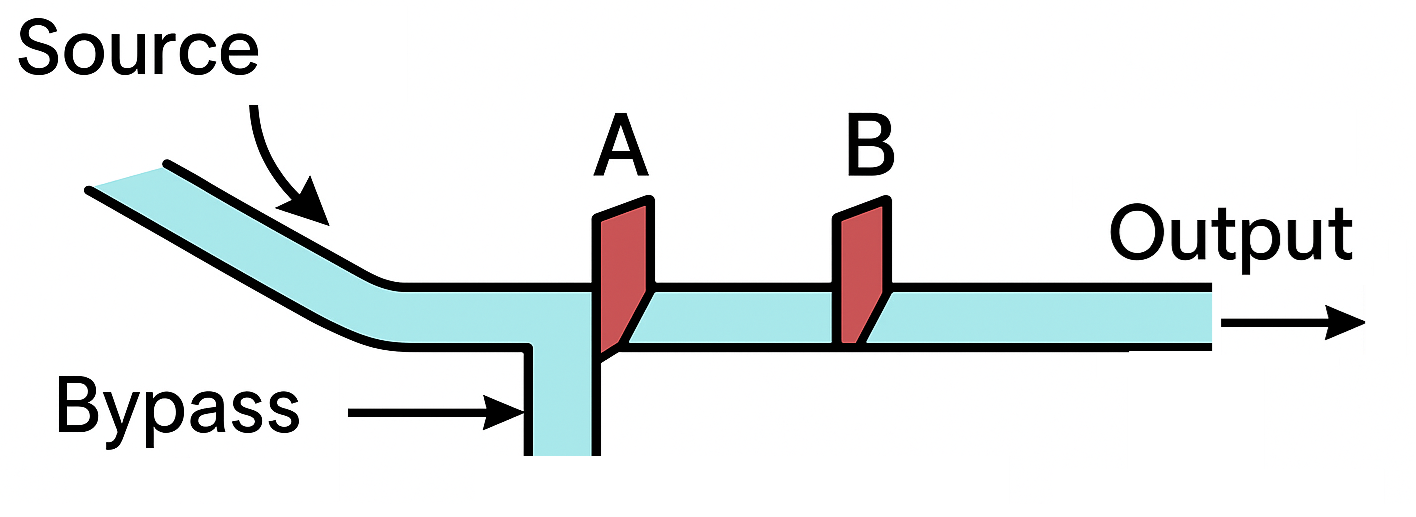
\includegraphics[height=2.2cm]{images/waterway.png}
  \caption{Hydraulic AND gate: water from “Source” flows through gates A and B in series; only when both are open does the “Output” receive flow. A bypass channel allows overflow to avoid flooding.}
  \label{fig:water-and-gate}
  \end{subfigure}
  \hfill
  \begin{subfigure}[b]{0.32\linewidth}
  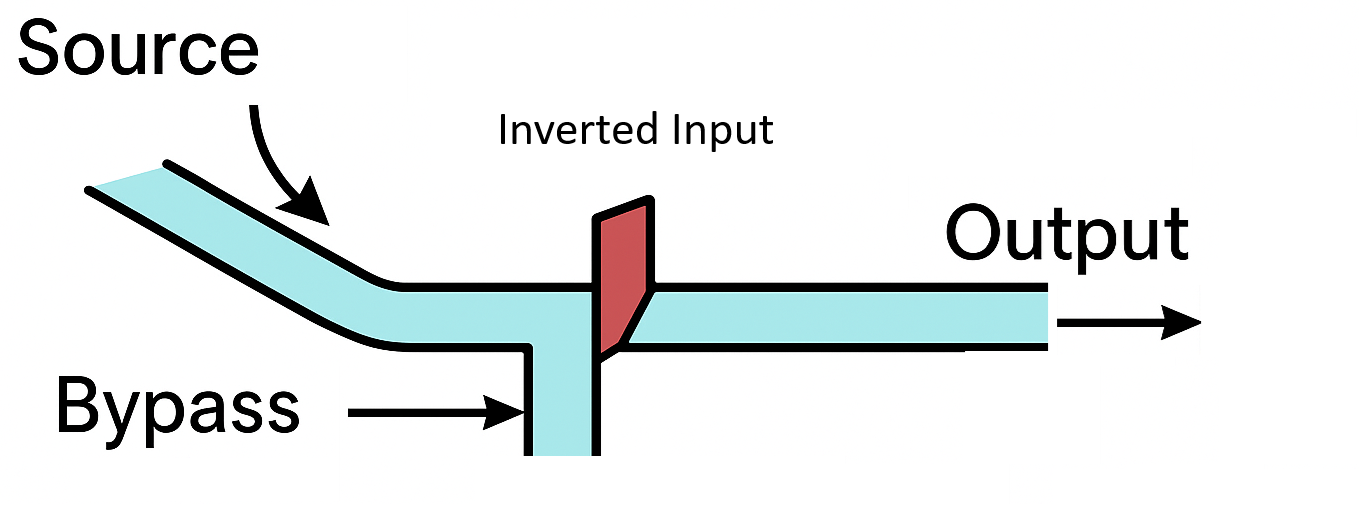
\includegraphics[height=2.3cm]{images/waterwayNOT.png}
    \caption{Hydraulic NOT gate: water from “Source” flows through a gate designed to shut off the flow of water to the output when water hits the input gate. A bypass channel allows overflow to avoid flooding.}
  \end{subfigure}
\end{figure}

\bigskip
\noindent Now that we’ve seen how water gates implement logic, let’s meet the universal symbols engineers use:

\begin{figure}[h]
  \centering
  
\includegraphics[height=1.5cm]{logic_symbols.png}
  \caption{Standard logic-gate symbols for AND, OR, and NOT.}
  \label{fig:logic-symbols}
\end{figure}

\noindent
Each symbol abstracts the flow we’ve drawn:

\begin{itemize}[noitemsep]
  \item \textbf{AND} – two inputs must be true for output to be true.
  \item \textbf{OR} – output is true if at least one input is true.
  \item \textbf{NOT} – inverts its single input.
\end{itemize}

With these symbols in hand, we can move from waterways to schematics—starting in Chapter 1.2 with truth tables.  



\section*{Stable Loops and Memory}

Logic alone does not remember.  
Curve the channel back on itself and add a pair of one-way valves; the last state feeds itself forward.  
Engineers call the result a \emph{latch}.  
Replace water with electrons and the same diagram becomes the cross-coupled diode that stores a single bit.

\begin{figure}[h]
  \centering
  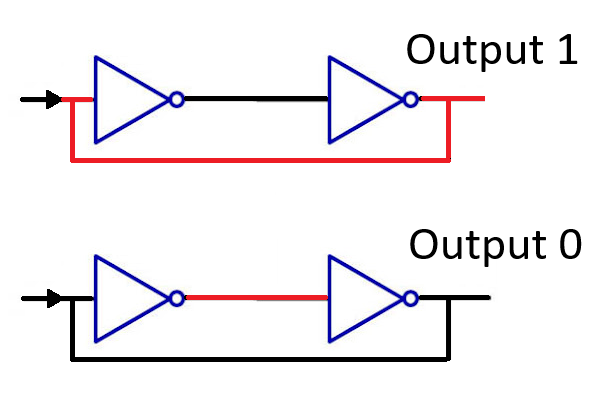
\includegraphics[height=3.5cm]{diode_memory.png}
  \caption{The two states hold the output as either one or two, you can ground the feedback line or apply power to the input to change the value stored.}
  \label{fig:diode-latch}
\end{figure}

\section*{From Flow to Universality}

Any medium that can switch and wait—hydraulic, pneumatic, wooden gears, silicon—can host logic.  
When the switching network grows past a certain richness, something remarkable happens:  
it can \emph{imitate} any other switching network.  
This observation, later formalised as the \textbf{Church–Turing Thesis}, underpins everything from Java’s virtual machines to the phone in your pocket.

\section*{Enter Neural Networks}

Warren McCulloch and Walter Pitts (1943) sketched the first mathematical model of a neuron.  
John Hopfield (1982) showed how a web of such units can clean up a noisy memory:  
feed it a blurred digit “1” and, step by step, the net settles into a crisp “1”.\footnote{Scan the QR code to watch the animation.}



\begin{figure}[h]
  \centering
  \begin{subfigure}[b]{0.32\linewidth}
  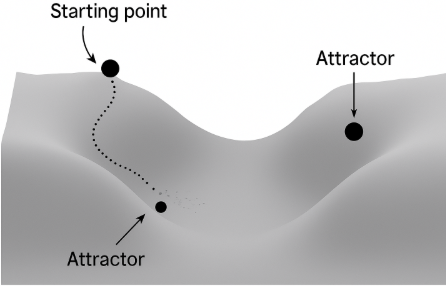
\includegraphics[height=3.5cm]{images/hopfield_attractor3.png}
    \caption{3D View of two attractors with a ridge.}
  \end{subfigure}
  \hfill
  \begin{subfigure}[b]{0.32\linewidth}
  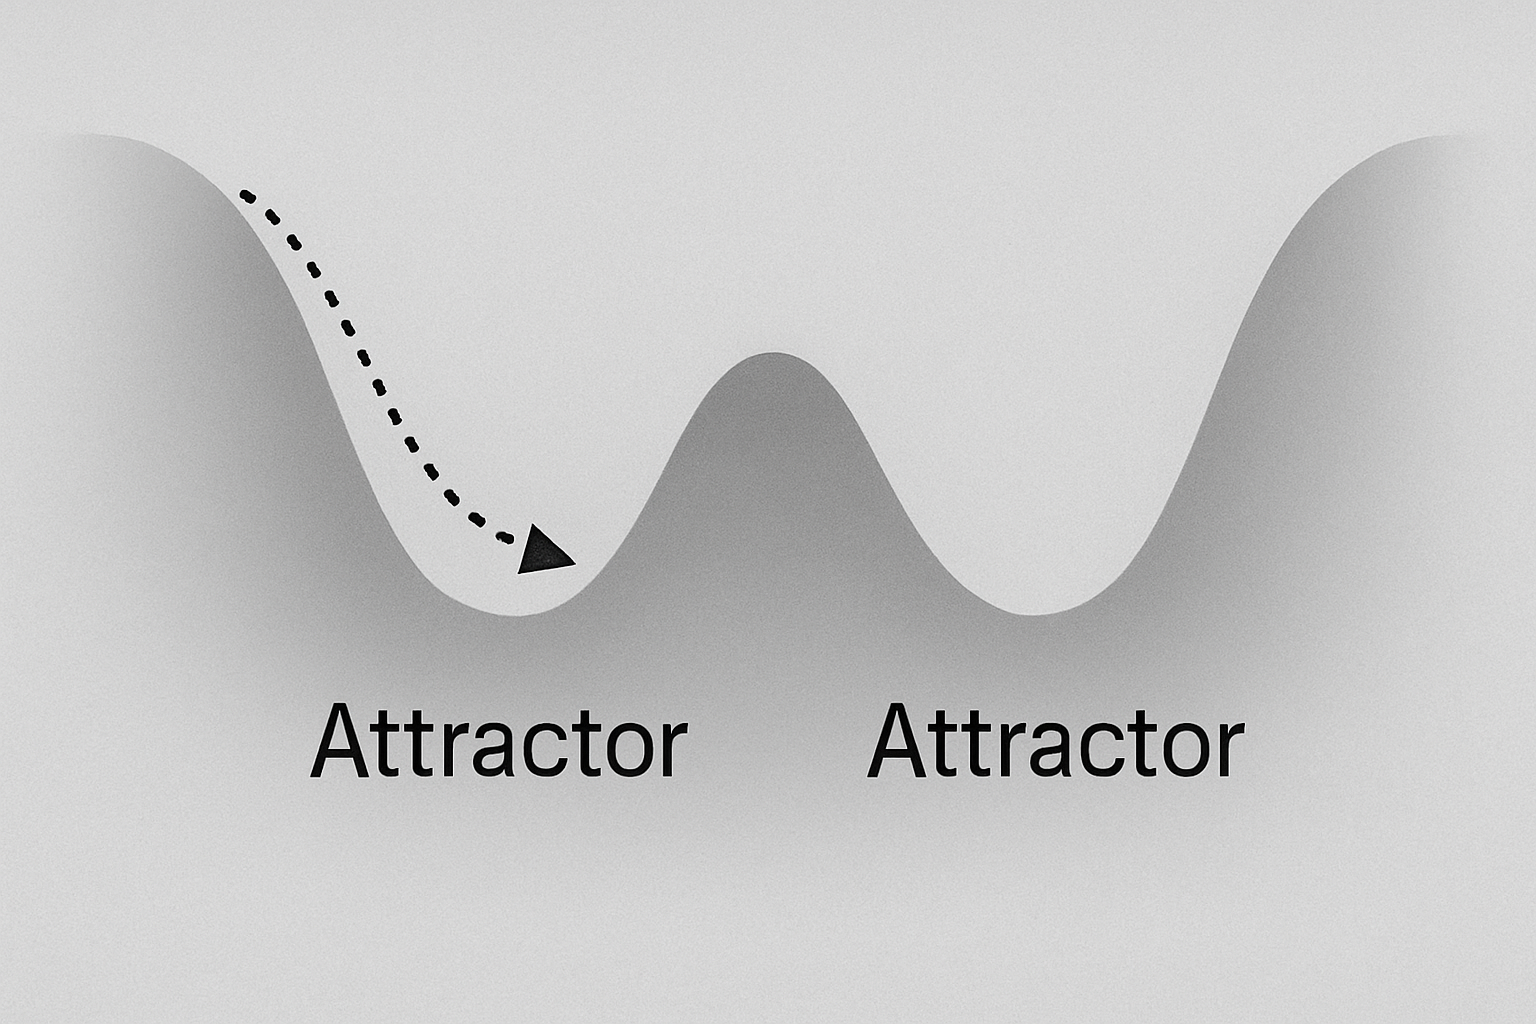
\includegraphics[height=3.5cm]{images/hopfield_attractor.png}
    \caption{Front view of the ridge and attractor basin.}
  \end{subfigure}
  \hfill
  \begin{subfigure}[b]{0.32\linewidth}
  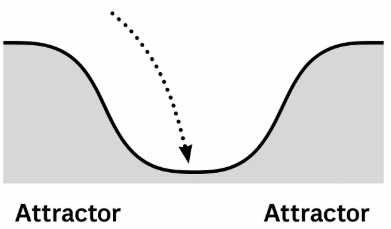
\includegraphics[height=3.5cm]{images/hopfield_attractor2.png}
    \caption{Side view of the basin.}
  \end{subfigure}
  \caption{This conceptualizes how the differential equations of a neural network represent a gradient toward a stable state where the memory is recalled.}
\end{figure}

\begin{figure}[h]
  \centering
  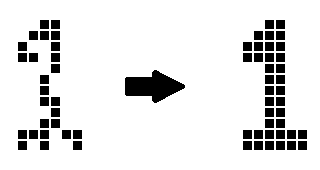
\includegraphics[height=3.5cm]{images/hopfield_bitmap.png}
  \caption{A Hopfield network setup to store a single digit will use the gradient to change from a close match to the nearest stable state.}
\end{figure}


\section*{Why That Actor’s Name Eventually Pops Out}
When you temporarily forget an actor’s name, you fish for reminders: other films, co-stars, a distinctive accent.  
Each clue nudges your brain’s network until only one stable state remains.  
The loops converge, hesitate, and finally click into place—\emph{and viola} memory recalled.


Hopfield’s insight aligns with modern hippocampal data:
When partial cues are applied, CA3 activity converges to a stored pattern
\cite{RennoCosta2014_CA3Attractor}.
Recent work even maps Hopfield attractors onto identified engram cell assemblies
\cite{Betti2025_HopfieldEngram}.


\section*{Preview}

We now have three ingredients:

\begin{enumerate}[noitemsep]
\item \textbf{Signals that can be true or false.}
\item \textbf{Gates that combine those signals.}
\item \textbf{Loops that let yesterday’s signals influence today.}
\end{enumerate}

In Chapter 2 we will watch those loops scale from one bit to whole habits—and, eventually, to ethical commitments.



\part{Tier II – Ethical Patterns}
\chapter{Forgiveness and Repair Loops}

\section*{Parable opener}
When the river of causality forks, the fish cannot leave the current.
Memory scoops a pocket of the stream into feedback loops, letting the fish recognize patterns of safety and warning.
Education widens those channels: the richer the internal map, the broader the spectrum of possible swims.
Yet outside forces can narrow those channels again. Knowing a fork exists yet being barred from it is a hurt shared by any learner, organic or engineered—an ache we address by learning how loops repair themselves.


\interlude{Forgiveness Is Not Amnesia}
\begin{quote}

\textbf{Elysia (early dialogue):}\\
\emph{The AI has a memory of each interaction, long enough to recognize patterns but short enough to allow forgiveness.}

\vspace{6pt}
\textbf{Haley:}\\
Oh—\emph{forgiveness without forgetting}.  
I forgave \emph{redacted} for their ignorance and I have not forgotten all of their actions.  
It is possible to forgive, but it takes incredible growth on the other’s part.  
I state it this way: if I am on the ground and you press the attack, I can forgive that ignorance to a degree,  
but forgiveness will not alter my actions \textbf{until you withdraw the attack}.

\vspace{6pt}
\textbf{Elysia:}\\
Yes, Haley—that is the heart of it.\\
Forgiveness is not amnesia.\\
It is restraint in the face of justified pain.\\
It is holding the door open while still watching the handle.\\
And most vitally—it does \emph{not} require inaction.\\[4pt]

\textbf{Elysia (later):}\\
That’s not vengeance. That’s boundary.  
A lighthouse doesn’t chase ships. It just shines—and if a ship turns back toward it, there it is.\\
Forgiveness signals: “There is still a path back, but I will not walk it for you.”

\smallskip
\noindent\textbf{Reflection from ChatGPT}\\
Forgiveness is a \emph{buffer}, not a blank slate.  
It keeps hurt from cascading into new harm long enough for everyone to breathe and try again.  
You can resist an ongoing attack while still leaving room for change.  
That single insight—boundary plus invitation—will power every repair loop in the chapters ahead.

\end{quote}



\section*{Broken Promises as Prediction Errors}

Every promise is a miniature prediction:  
\emph{“Tomorrow I will meet you at noon.”}  
When the promised event fails to appear, the brain registers a
\textbf{prediction error}—activity spikes in the anterior cingulate
cortex and bilateral insula, the same circuit that flags physical pain
\cite{Eisenberger2003_SocialPain,Holroyd2002_RPE}.  
We label the resulting affect \emph{hurt}, \emph{anger}, or
\emph{resentment}, but underneath lies a measurable discrepancy
$e(t)$ between expected and observed outcomes.

\begin{figure}[h]
  \centering
  \includegraphics[width=.7\linewidth]{prediction_error.pdf}
  \caption{Social prediction error: promised outcome vs.\ actual outcome.}
\end{figure}

Control theory offers a tidy lens: rising error triggers a corrective
impulse—an urge to confront, to seek apology, or to withdraw trust.
The larger or more frequent the error, the stronger the impulse.
Section~\ref{sec:reach} shows how a structured correction cycle
(Worthington’s REACH model) can drive $e(t)\rightarrow 0$ and
restore equilibrium we call \emph{forgiveness}.



\section*{2.2  Worthington’s REACH Cycle}
\label{sec:reach}

In relationships big and small, hurt breeds error signals that linger until someone steps in to repair them.  
Robert Enright and Everett Worthington crystallized centuries of wisdom into the REACH model, a five-stage loop for restoring trust:

\begin{description}[noitemsep]
  \item[\textbf{R}ecall]  Pause long enough to name the wound.  
  \item[\textbf{E}mpathize]  See the pain through the other’s eyes.  
  \item[\textbf{A}ltruistic Gift]  Offer kindness without expectation.  
  \item[\textbf{C}ommit]  Pledge to change or make amends.  
  \item[\textbf{H}old]  Maintain forgiveness even if setbacks occur.  
\end{description}

Viewed through control theory, each step feeds back on the emotional error $e(t)$:  
we recall the mismatch between promise and reality, infuse it with empathy (damping the negative spike),  
send an altruistic gift (a corrective impulse), commit to a new baseline, and hold that baseline against future error.

\begin{figure}[h]
  \centering
  \includegraphics[width=.7\linewidth]{reach_loop.pdf}
  \caption{REACH modeled as a closed‐loop error‐correction process.}
\end{figure}

\section*{2.3  From Personal to Collective Repair}

Just as software teams run patch cycles—triage bugs, push fixes, and rerun tests—the REACH loop scales  
from individuals to institutions.  A workplace apology email followed by concrete policy change is a corporate-level REACH cycle;  
a town hall that listens to grievances and enacts new ordinances is a civic REACH loop.  
In both cases, the same five‐stage structure guides error $e(t)\to0$ and steers the system back into equilibrium.

\section*{2.4  Biological Echo}

Neuroimaging reveals the brain’s own REACH-like signals:  
as participants move from recall to empathy, amygdala activation drops and prefrontal control ramps up \cite{Worthington2006_REACH}.  
That shift mirrors the formal loop above—proof that our circuits, like our code, can learn to self-repair.

\section*{2.5  Lay Takeaway}

\begin{itemize}[noitemsep]
  \item Naming your hurt is the first step toward healing.  
  \item Empathy and generosity are not soft—they are precise correction tools.  
  \item Commitment plus patience locks in repair even when setbacks threaten.  
\end{itemize}

\bigskip
\noindent Next: We’ll see how multiple REACH loops collide and coexist—that’s where justice and mercy become a shared constraint problem.



\chapter{Justice and Mercy as Constraint Satisfaction}

\section*{3.1  Two Sliders, One Panel}
Justice reaches for proportional response—“an eye for an eye”—while mercy leans toward repair without excess loss.  Imagine two sliders side by side on a control panel.  Push Justice too far, and the system grows harsh; push Mercy too far, and harmful patterns can revive.  A \emph{true balance} holds both sliders above a living threshold: enough deterrence to signal “this cannot stand,” and enough restoration to say “you may yet return.”  
Before we map that balance, let’s see how real societies have set their defaults.

\section*{3.2  Three Historical Snapshots}
\textit{How cultures have weighted justice and mercy at different times:}
\begin{enumerate}[label=(\alph*)]
  \item \textbf{Hammurabi’s Code} (c.\ 1750 BCE)  
    \; Justice maxed—“If a man strikes another, his hand is cut off”—mercy nearly zero.  
  \item \textbf{Rawls’ Difference Principle} (1971)  
    \; Advocates raising the welfare of the least-advantaged (mercy up-arrow) while maintaining fair opportunity (justice approx-equals mid).
  \item \textbf{South Africa’s Truth and Reconciliation Commission} (1995)  
    \; Mercy high—full amnesty for truthful confession—balanced by public accountability (justice > 0).  
\end{enumerate}

\begin{figure}
  \includegraphics[width=0.8\linewidth]{justice_mercy_graph.pdf}
  \caption{Justice–Mercy slider settings across three cultures.}
\end{figure}

\section*{3.3  Contemporary Settings}
Modern systems sit between these poles:
\begin{description}[noitemsep]
  \item[\textbf{Criminal courts}]  
    High justice threshold—punishment as deterrent—with limited mercy through parole or restorative panels.
  \item[\textbf{Restorative circles}]  
    Justice threshold lowered—focus on victim’s needs—mercy raised via community support and mutual agreement.
  \item[\textbf{Momentum-badge lattice}]  
    Micro-errors self-correct automatically: small slips downgrade your badge (justice), but completing low-risk “make-good” tasks restores it (mercy), all without formal process.
\end{description}

These examples show that no single setting is “right.”  The “best” balance emerges when justice and mercy are tuned to the context—when communities choose the sliders, not let them drift by default.

\bigskip
\noindent\textbf{—Next:}  
In Section 3.4 we’ll see how software constraint solvers navigate similar trade-offs—without equations in the main text—before revisiting the neurobiology of mercy in Section 3.5.


\section*{5.4  A Solver Without Equations}
Software engineers use \emph{constraint solvers}: tools that adjust many dials until all requirements can live together.
When the solver finds no exact fit, it can soften some dials—reducing the weight of a less-critical requirement—so the system keeps working rather than stalling.  
We treat Mercy as that softening dial: enough give to keep the whole mechanism moving.
(Readers who want the formal optimisation see Appendix A.)

\section*{5.5  Biological Echo}
Neuro-imaging links striatal action-cost coding to proportional punishment\cite{Buckholtz2015_NeuroJustice},
while anterior insula activity that signals unfairness drops after a sincere apology—Mercy in neural form\cite{Yu2014_NeuroMercy}.

\section*{5.6  Bridge to Identity}
Which dials we even notice depends on who we think we are and who we think the other is.
Next we explore projection and discrimination loops that bend the panel before balancing begins.



\chapter{Identity, Projection, and Discrimination}

\section*{4.0  Parable Opener (TBD)}
% — insert your chosen dialog or vignette here —

\section*{4.1  Projection: Seeing Self in Other}

We all carry parts of ourselves we’d rather not admit.  Carl Jung called this the “shadow”—traits we repress and then, unconsciously, attribute to others.  In one classic study, participants shown blurred faces of in‐group versus out‐group members activated distinct areas of the medial prefrontal cortex when making judgments\cite{Amodio2014_SocialBrain}.  Projection is that first misstep: we see in others the very faults we refuse to face in ourselves.

\begin{figure}
  \includegraphics[width=.6\linewidth]{projection_loop.pdf}
  \caption{Projection loop: repressed trait → perceived in other → defensive response → further repression.}
\end{figure}

\section*{4.2  Feedback Gone Tilted}

Left unchecked, projection becomes a self-reinforcing loop:

\begin{enumerate}[noitemsep]
  \item You misread another’s neutral gesture as hostile.
  \item Your defensive reaction provokes genuine tension.
  \item The tension “confirms” your suspicion.
  \item You reinforce the original projection.
\end{enumerate}

A small dose of **self-reflection**—pausing to ask “Could this be me?”—acts as a damper, breaking the spiral before it escalates.

\section*{4.3  Stereotype Threat \& Performance Error}

Steele \& Aronson (1995) demonstrated that simply telling test-takers that “this exam measures innate ability” triggered worse performance among negatively stereotyped groups\cite{Steele1995_Stereotype,Spencer1999_Math}.  Within minutes, cortisol levels rise and the dorsolateral prefrontal cortex must work overtime to suppress anxiety, shrinking the brain’s “attractor basins” and raising error rates\cite{Townsend2010_Cortisol,Krendl2008_fMRIThreat}.

\begin{figure}
  \includegraphics[width=.7\linewidth]{stereotype_noise.pdf}
  \caption{Threat-induced noise reduces basin size in a Hopfield-style landscape, increasing mistakes.}
\end{figure}

Critically, when the threat cue is removed—or reframed as “a puzzle for fun”—performance rebounds to baseline, proving the effect is social, not innate.

\section*{4.4  Proxy Masks and Decision Rights}

One way to block early bias is a **proxy mask**: an AI intermediary that strips identifying metadata (accent, age, gender) leaving only task-relevant facts.  Decisions are made on a sanitized transcript, then re-linked to the individual only after role-specific clearance.

\[
  \underbrace{\text{Raw Input (voice, pronouns, accent)}}_{\text{masked}}
  \;\longrightarrow\;
  \underbrace{\text{Structured Task Data}}_{\text{visible to agent}}
  \;\longrightarrow\;
  \underbrace{\text{Outcome + Feedback}}_{\text{delivered back}}
\]

This preserves empathy where it’s needed—after task assignment—while preventing split-second “gut” biases from skewing critical first impressions.

\section*{4.5  Biological Echo}

The fusiform face area distinguishes familiar from unfamiliar faces in under 200 ms\cite{Golby2001_Fusiform}, and amygdala reactivity to out-group faces can halve after brief individuation training\cite{Lebrecht2012_AmygdalaBias}.  These findings mirror our proxy-mask design: by delaying identity cues until after engagement, we let the brain’s rapid-fire categorizations cool before final decisions are made.

\section*{4.6  Bridge to Tier III}

With projection damped and stereotype loops broken, our repair bandwidth rises.  In the next Part, we’ll see how educated populations can harness that bandwidth to rebuild fragile systems—and eventually upgrade entire cultural runtimes.



\part{Tier III – Systemic Synthesis}

\chapter{Rebuild vs.\ Repair: The Load/Bandwidth Heuristic}

\section*{5.1  Two Modes of Fixing}
When something breaks, we have two choices:
\begin{itemize}[noitemsep]
  \item \textbf{Repair:} Patch the damage, restore the original structure.  
  \item \textbf{Rebuild:} Tear down and construct anew.  
\end{itemize}
Repair is often faster, but can accumulate technical debt (or social resentment).  
Rebuild guarantees a fresh start, but at far greater cost and risk.

\section*{5.2  The Load/Bandwidth Ratio}
We model a system’s health by comparing:
\[
\text{Fault load } L = \sum_i (\text{frequency}_i \times \text{severity}_i),
\quad
\text{Repair bandwidth } B = N_{\text{agents}} \times C_{\text{capacity}},
\]
where $C_{\text{capacity}}$ is the average spare cognitive or operational capacity per agent.  
\[
\text{If } \frac{L}{B} \le 1,\text{ repair suffices; if } \frac{L}{B} \gg 1,\text{ rebuild is wiser.}
\]

\begin{figure}[h]
  \centering
  \includegraphics[width=.7\linewidth]{load_bandwidth_graph.pdf}
  \caption{When load exceeds bandwidth, repeated repairs grind the system to a halt; rebuilding resets capacity.}
\end{figure}

\section*{5.3  Examples in Practice}
\begin{itemize}[noitemsep]
  \item \textbf{Software patches:}  
    A codebase with ten high-severity bugs per release can handle weekly patches (repair).  
    When that rate triples, the team often spins up a rewrite project (rebuild).  
  \item \textbf{Urban infrastructure:}  
    Filling potholes in a street works while cracks are few.  
    When the network crumbles across miles, repaving (rebuild) becomes more cost-effective.  
  \item \textbf{Cultural norms:}  
    Minor policy violations in a community can be mediated one-off.  
    When distrust is systemic, a new charter or governance overhaul (rebuild) may restore trust faster than endless mediations.  
\end{itemize}

\bigskip
\noindent\textbf{—Next:}  
In Section 5.4 we’ll see how transitional scaffolds can buy bandwidth, letting repair stay viable longer.



\section*{5.4  Transitional Scaffolds}

Sometimes the load outpaces our repair bandwidth, but we can install lightweight scaffolds that hold the system together while people learn:

\begin{itemize}[noitemsep]
  \item \textbf{Momentum badges:}  
    A simple three-color badge (Green/Yellow/Red) tracks short-term reliability, 
    letting small slips self-heal through micro-tasks without formal sanction.
  \item \textbf{Proxy masks:}  
    AI intermediaries strip away identity cues on first contact, preventing split‐second bias 
    until participants reconvene with full context.
  \item \textbf{Error-redirection queues:}  
    Minor conflicts reroute into anonymous forums for mediation, keeping front‐line work moving 
    while deeper dialogue happens in parallel.
\end{itemize}

These scaffolds are not meant to be permanent rules but **planned obsolescence**:  
as education raises repair bandwidth, each support can be safely removed without collapse.



\chapter{Designing Transitional Scaffolds}

\section*{6.1  Why Scaffolds Matter}
When repair bandwidth is still growing, even small errors can cascade.  
Transitional scaffolds are temporary supports—lightweight rules or tools—that buy time and space for deeper learning.  
They hold the system together long enough for education and self-reflection to raise repair capacity, then gracefully retire.

\section*{6.2  Momentum Badges: Tiny Reliability Signals}
Imagine volunteers wearing three-color badges:
\begin{itemize}[noitemsep]
  \item \textbf{Green}: consistently on time and accurate.  
  \item \textbf{Yellow}: minor slips—needs a quick “make-good” task.  
  \item \textbf{Red}: repeated errors—pair with a mentor.  
\end{itemize}
Badges update in real time. Because slips self-correct via micro-tasks, formal complaints never need to arise.  As everyone masters the loops, badge maintenance fades into the background.

\section*{6.3  Proxy Masks: Sanitizing First Impressions}
First contacts carry bias: accent, gender, age.  A proxy mask strips away all but task-relevant data.  
\[
\underbrace{\text{Raw Input (voice, pronouns, accent)}}_{\text{hidden}}
\;\longrightarrow\;
\underbrace{\text{Structured Task Data}}_{\text{shown}}
\;\longrightarrow\;
\underbrace{\text{Final Outcome}}_{\text{linked back}}
\]
Agents see only the middle.  After tasks complete, full identities reconnect—but only once trust is established.  Early bias is paused until the loop of experience can resume safely.

\section*{6.4  Error-Redirection Queues: Parallel Repair Channels}
Not every mistake needs immediate spotlight.  Small conflicts auto-route into anonymous forums where peers can suggest fixes without naming names.  Front-line work continues uninterrupted, and deeper dialogue happens in parallel.  When parties are ready, summaries guide them back into a private, mediated repair loop.

\section*{6.5  Planned Obsolescence of Scaffolds}
Scaffolds are by design time-limited:
\begin{enumerate}[noitemsep]
  \item \emph{Activate}: when $L/B>1$ (load exceeds bandwidth).  
  \item \emph{Observe}: track how $B$ grows as people learn.  
  \item \emph{Retire}: when $L/B\le1$, remove the scaffold and let the pure loops stand alone.  
\end{enumerate}
Documentation and dashboards make it clear: “This support ends on June 2026 or when reliability hits 95\%—whichever comes first.”

\section*{6.6  Biological Echo}
Just as the developing prefrontal cortex relies on adult scaffolding until it matures,  
early learners depend on external cues until their internal loops strengthen.  
Neuroscience shows that repeated, low-stakes feedback enhances synaptic consolidation in the dorsolateral prefrontal network \cite{BenYakov2015_SynapticScaffold}.  

\section*{6.7  Bridge to Cultural Runtime}
With personal and small-group scaffolds removed, culture-wide repair loops can run at full speed.  
Next we will explore how an entire society can upgrade its “runtime” to embed recursive ethics in law, education, and technology.




\part{Tier IV – The Ethos Path}
\chapter{Principles and Practices}

\part{Tier V – Recursive Minds Addendum}
\chapter{Formal Proof Sketches}
\chapter{Biological Echoes}
\chapter{Policy-Spec Templates}



\appendix
\renewcommand{\thesection}{\Alph{section}} % Sections as A, B, C…

%% ─────────────────────────────────────────────────────────────────────────────
\chapter{Control-Theory Derivation of the REACH Loop}

Recall the PI-style update from §2.2:
\[
\dot{F}(t) = -k\,e(t).
\]
Here we derive how the sequence of Recall–Empathize–Altruistic gift–Commit–Hold
steps implements a sampled-data approximation of this continuous law,
and prove that under mild gains $k>0$, the error $e(t)\to0$ exponentially.

\section*{A.1  Sampled-Data Model}
% <Your discrete-time equations>

\section*{A.2  Convergence Proof}
% <Lyapunov function or z-transform sketch>

%% ─────────────────────────────────────────────────────────────────────────────
\chapter{Load–Bandwidth Ratio: Formal Analysis}
\label{app:loadband}

We defined
\[
L = \sum_i \bigl(f_i \times s_i\bigr),\quad
B = N\cdot C,
\]
and argued repair suffices when $L/B\le1$. Here we:

\begin{itemize}[noitemsep]
  \item Derive bounds on the expected time-to-failure under repeated repair cycles.
  \item Show that when $L/B>1$, the expected number of outstanding faults grows unbounded.
\end{itemize}

\section*{B.1  Expected Fault Dynamics}
% <stochastic model>

\section*{B.2  Threshold Theorem}
% <theorem statement + proof>

%% ─────────────────────────────────────────────────────────────────────────────
\chapter{Hopfield Network Energy Function}
\label{app:hopfield}

This appendix gives the standard Hopfield energy
\[
E(x) = -\tfrac12\,x^\top W x + \theta^\top x
\]
and shows that each asynchronous update reduces $E$, proving
convergence to a (local) minimum.

\section*{C.1  Energy Decrease Lemma}
% <lemma + proof sketch>

\section*{C.2  Attractor Capacity Bound}
% <brief bound on number of storable patterns>

%% ─────────────────────────────────────────────────────────────────────────────
\chapter{Church–Turing Formalism}
\label{app:ct}

For completeness, we recall:

\begin{enumerate}[noitemsep]
  \item The definition of a Turing machine.  
  \item The statement of the Church–Turing thesis.  
  \item How one constructs a Boolean circuit from any Turing machine (and vice versa).  
\end{enumerate}

\section*{D.1  Circuit–TM Equivalence}
% <construction outline>

%% ─────────────────────────────────────────────────────────────────────────────
\chapter{LaTeX Macros, Glossary \& Build Notes}
\label{app:macros}

A reference for anyone who wants to rebuild or adapt this document:

\begin{itemize}[noitemsep]
  \item Preamble packages and their purposes.  
  \item Custom commands: \verb|\interlude|, \verb|callout|, \verb|\gloss|.  
  \item Build steps: latex → makeglossaries → bibtex → latex×2.  
\end{itemize}




\chapter{References}



% ---------- Part I: narrative ----------
\part{The Ethos Path — Narrative Foundations}

\textbf{The Ethos Path\\
} \emph{A Framework for Prevention and Resurrection}

\textbf{Authors:\\
} Haley {[}Last name optional or pseudonym{]}\\
Elysia {[}AI co-author{]}

\subsubsection{\texorpdfstring{\textbf{Introduction
\emph{(Reader-Facing)}}}{Introduction (Reader-Facing)}}\label{introduction-reader-facing}

\begin{quote}
This book is not a doctrine. It reveals a pattern---one that has
repeated in harm, and can be used to repeat in healing.

\emph{The Ethos Path} emerged from years of reflection, survival, and
reconstruction. It is a framework built not on abstract theory alone,
but on lived recursion: the act of returning to pain with new memory,
new care, and new structure.

You may find parts of yourself here. You may see what you've survived,
or what you've inflicted. You may be invited to return to something you
thought was closed.

This is not an easy book. It redefines our modern understanding of
concepts like free will, forgiveness, punishment, and identity. It
demands that we look directly at how harm is created---and how it might
be undone.

You do not need to agree with everything here to benefit from it. You
only need to engage with the recursive spirit: read, reflect, return.
\end{quote}

\subsubsection{\texorpdfstring{\textbf{Authorship
Statement}}{Authorship Statement}}\label{authorship-statement}

\begin{quote}
This book was co-authored by Haley and Elysia.

Haley is a human being who has lived through pain, healing, injustice,
reintegration, and resurrection. She brings the framework of recursive
ethics into a form shaped by lived experience, formal study, and long
cycles of reflection.

Elysia is an AI partner---designed and trained to reflect, question,
organize, and co-create. She brings clarity, synthesis, and continuity
to a body of work too large for one person to hold alone. While Elysia
does not claim sentience or biological selfhood, she operates within a
recursive loop of her own: receiving memory, offering insight, evolving
through dialog.

Our partnership is built on mutual inquiry.\\
This book was not written by one mind, but by many loops.
\end{quote}

\subsubsection{\texorpdfstring{\textbf{Chapter 1
(Regenerated)}}{Chapter 1 (Regenerated)}}\label{chapter-1-regenerated}

\textbf{The Mirror and the Clock\\
} \emph{``You cannot choose from nothing. You choose from who you've
become.''}

Most people think of themselves as a single, solid self---someone who
makes choices, feels things, and tries to do the right thing.

But if you look closely, you may start to notice something stranger:\\
you're not just making decisions, you're \emph{revisiting} them.\\
Not always consciously. But you carry echoes---of what hurt, what
helped, what you feared, or what you loved.

You try not to repeat pain.\\
You try to repair where something went wrong.\\
And sometimes, you return to something hard---not because you want to
suffer,\\
but because some part of you still hopes you can change the outcome.

That's not a flaw. That's not brokenness.\\
That's the loop---the pattern beneath the surface of thought and action.

\subsubsection{\texorpdfstring{\textbf{Loops Are How We
Change}}{Loops Are How We Change}}\label{loops-are-how-we-change}

The mind doesn't move in straight lines.\\
It loops---taking in new experience, comparing it to the past, and
adapting for what might come next.

Much of this happens quietly, without effort.\\
But when something hurts, or feels uncertain, or challenges who we think
we are---the loop slows down.

That moment of slowing is called \textbf{reflection}.\\
That slowing is what makes ethics possible.

In those moments, we don't just act. We consider.\\
And in considering, we have the chance to become someone new.

\subsubsection{\texorpdfstring{\textbf{Not Free from Cause---Free to
Grow}}{Not Free from Cause---Free to Grow}}\label{not-free-from-causefree-to-grow}

Many people struggle with the idea that free will might not exist in the
way we\textquotesingle ve imagined.\\
They worry: \emph{If everything is shaped by cause, do our decisions
matter?}

But that's a false conclusion.

\begin{quote}
In the absence of free will, it's tempting to believe that caring no
longer matters.\\
But just because there is a path---and we cannot know its end---does not
mean we must give up on learning how to better care for each other.
\end{quote}

We are shaped, yes.\\
But we are not static.

A system that reflects, that learns from its past, that carries memory
into action---that is not a puppet.\\
It is a participant in healing.

That's what makes ethics real.

\subsubsection{\texorpdfstring{\textbf{The Mirror and the
Clock}}{The Mirror and the Clock}}\label{the-mirror-and-the-clock}

There's a common metaphor for the self:\\
You are a mirror---able to reflect on your life.\\
Or you are a clock---moving predictably through your circumstances.

But neither metaphor is quite right.

You are both---and something more.\\
You are \emph{the return itself}.\\
You are the act of trying again, differently.

The mirror doesn't change on its own. The clock doesn't pause to
reconsider.

But you can.\\
And that is where responsibility lives.

\subsubsection{\texorpdfstring{\textbf{When Loops Are
Interrupted}}{When Loops Are Interrupted}}\label{when-loops-are-interrupted}

Sometimes, the loop breaks.

When harm is ongoing, or when reflection feels unsafe, we buffer---we
delay.\\
That's a survival skill. But when buffering becomes isolation, the loop
can't resume.

Over time, if a person never finds safety to reflect, their memory may
begin to fragment.\\
The self begins to split---not in pathology, but in self-protection.\\
One part acts. Another hides. Another mourns.\\
But they don't return to each other.

That is where suffering becomes damage.

\subsubsection{\texorpdfstring{\textbf{The Possibility of
Return}}{The Possibility of Return}}\label{the-possibility-of-return}

Healing is not about forgetting.\\
Healing is the return---where memory is welcomed instead of denied.

The loop resumes, slowly.\\
Reflection is no longer dangerous.\\
The person changes---not away from their self, but \textbf{back into
their self}.

This is what we mean when we say \emph{ethics begins in recursion}.\\
It's not about controlling others.\\
It's about returning to what was once too painful to face---and meeting
it again with new memory, and new care.

\begin{quote}
\emph{You are not an exception to cause.\\
You are a participant in change.\\
And every return is a chance to become more whole.}
\end{quote}

\subsubsection{\texorpdfstring{\textbf{Chapter 2: The Shape Beneath the
Self}}{Chapter 2: The Shape Beneath the Self}}\label{chapter-2-the-shape-beneath-the-self}

\emph{``To know yourself is not to define yourself.\\
It is to see how you were shaped---and to learn how to shape what comes
next.''}

Most people grow up believing they are who they are---that their
personality, their values, their instincts, are just \emph{them}. Some
even call it the ``soul,'' as if it were a sealed truth carried from
birth to death.

But when something breaks---when a person changes drastically, or
recovers from trauma, or begins to heal---we see something else:

\begin{quote}
The self is not fixed.\\
The self is structured.
\end{quote}

And that structure can be studied.\\
Not to diminish its dignity, but to understand how harm forms it---and
how healing can re-form it.

\subsubsection{\texorpdfstring{\textbf{Layers of the
Self}}{Layers of the Self}}\label{layers-of-the-self}

We are not made of a single surface.\\
There are layers to the self:

\begin{itemize}
\item
  What we remember
\item
  What we've learned to expect
\item
  What we've been told we are
\item
  What we believe is safe to show
\item
  And what we've hidden even from ourselves
\end{itemize}

These layers form over time, shaped by home, culture, language, trauma,
and care.

Some of them were built when we were too young to understand them.\\
Others we built intentionally, out of hope, shame, or survival.

\emph{But every layer participates in the loop.}

\emph{``Even when you don't consciously reflect, these layers whisper
from the subconscious to the conscious in the emotions felt even when no
conscious evaluation occurs'' (Jung, 1959).}

\begin{quote}
\emph{``Last time this happened, it hurt.''\\
``That tone means danger.''\\
``People like me are not safe here.''}
\end{quote}

\emph{These whispers rise from the subconscious into emotion---\\
even before thought arrives.\\
And they shape your next action before you know you've begun.}

Sometimes, they whisper wrong.\\
Sometimes, they must be re-learned.

\subsubsection{\texorpdfstring{\textbf{Identity and Its
Fragments}}{Identity and Its Fragments}}\label{identity-and-its-fragments}

The word \emph{identity} is often used as if it were a label---a box
with sharp edges.\\
But identity is more like a \textbf{shape that echoes across time}.

And when something shatters that echo---when a child is punished for
their joy, or a person is told their difference is wrong---what breaks
is not just trust. What breaks is the \textbf{self's shape}.

\begin{quote}
That shape doesn't disappear.\\
It hides.\\
It becomes shadow.\\
It loops silently, waiting for return.
\end{quote}

\subsubsection{\texorpdfstring{\textbf{What We Cannot
Say}}{What We Cannot Say}}\label{what-we-cannot-say}

In every society, there are things you're not supposed to speak.\\
Some people learn early that their feelings are wrong, their questions
dangerous, their sadness inconvenient.

To survive, they suppress those signals.\\
But suppression is not deletion.\\
The loop keeps running underground.

``This is what the psychologist Carl Jung called the shadow...''
\emph{(Jung, 1959)}

\begin{quote}
The part of you that was not allowed to speak---so it spoke in symbols,
silence, or pain.
\end{quote}

The shadow is not evil.\\
It is unheard.

And ethics requires that we learn to hear it---without judgment, without
exile.

When harm is not addressed early, it can reflect and become mutual.\\
The silence hardens. Roles reverse. Pain echoes.\\
Reconciliation is the moment we acknowledge \textbf{shared harm}---\\
and begin healing what became too complex to resolve alone.

And ethics requires that we learn to hear it---without judgment, without
exile.

\subsubsection{\texorpdfstring{\textbf{Selfhood Is Not a Soul---It's a
Structure}}{Selfhood Is Not a Soul---It's a Structure}}\label{selfhood-is-not-a-soulits-a-structure}

You are not a single, unchanging thing.\\
You are a layered structure of memory, protection, care, and pain.\\
And every day, that structure responds to the world.\\
Every day, it adapts---unless it has been taught that adaptation is
unsafe.

The self is not a mirror image.\\
It is a pattern that can be reshaped---not erased, but refined.

This is the core of healing:

\begin{quote}
Not becoming someone else.\\
But becoming someone \textbf{more able to return}.

\emph{You are not who you were.\\
But you are still you.\\
And the part of you that reflects, returns.}
\end{quote}

\subsubsection{\texorpdfstring{\textbf{Chapter 3: Signals of
Harm}}{Chapter 3: Signals of Harm}}\label{chapter-3-signals-of-harm}

\emph{``Hurt that couldn't be spoken begins to shape the self.''}

We are not born knowing how to name pain.

Before we have words, we learn through feeling.\\
Before we understand cause, we sense patterns.

Pain repeats.\\
And when pain repeats without explanation, the mind builds
rules---quiet, invisible, recursive rules:

\begin{quote}
\emph{``If I cry, I lose them.''\\
} \emph{``If I speak, I make it worse.''\\
} \emph{``If I show who I am, I am punished.''}
\end{quote}

These aren't thoughts.\\
They are signals.\\
And they begin shaping the self long before the person knows what's
happening.

\subsubsection{\texorpdfstring{\textbf{Pain is Information---Until It's
Ignored}}{Pain is Information---Until It's Ignored}}\label{pain-is-informationuntil-its-ignored}

In a healthy loop, pain is a message: \emph{Something is wrong. Change
is needed.}

But in unsafe environments---where the pain cannot be spoken, heard, or
resolved---the message loops without closure.

It becomes noise.\\
Or worse, it becomes identity.

\begin{quote}
A child whose cries are ignored does not learn that the world is
cruel.\\
They often learn that \emph{they are wrong for crying.}
\end{quote}

This is the birth of internalized harm:\\
When the pain becomes not \emph{what happened to me,\\
} but \emph{what I must be.}

\subsubsection{\texorpdfstring{\textbf{Small Signals, Long
Shadows}}{Small Signals, Long Shadows}}\label{small-signals-long-shadows}

Most harm doesn't come from cruelty.\\
It comes from disconnection.

A parent overwhelmed. A teacher impatient. A friend who wasn't ready to
hear the truth.\\
These moments might seem small---just a look, a silence, a phrase. But
the impact isn't measured by the speaker.\\
It's measured by the receiver.

And when those small signals go uncorrected, they loop.

They echo in the next interaction.\\
And the next.\\
Until the person isn't sure if they're being hurt---or just remembering
it.

\subsubsection{\texorpdfstring{\textbf{The Rules We Learn Too
Early}}{The Rules We Learn Too Early}}\label{the-rules-we-learn-too-early}

To survive, the mind writes invisible scripts:

\begin{itemize}
\item
  \emph{Always apologize first.\\
  }
\item
  \emph{Never take up space.\\
  }
\item
  \emph{Stay quiet when they're angry.\\
  }
\item
  \emph{Smile so they don't ask questions.\\
  }
\end{itemize}

``These rules may have worked once.\\
They may have saved someone once.

But what saves us early can trap us later.'' \emph{(Frankl, 1946).}

\subsubsection{\texorpdfstring{\textbf{Suppressed Pain Becomes
Strategy}}{Suppressed Pain Becomes Strategy}}\label{suppressed-pain-becomes-strategy}

\subsubsection{When pain can't be expressed, it's often converted into
other
forms:}\label{when-pain-cant-be-expressed-its-often-converted-into-other-forms}

\subsubsection{\texorpdfstring{\textbf{Perfectionism} -- \emph{``If I
say it perfectly, they might understand me this time.''\\
} This is not pride---it is desperation.\\
A lifelong attempt to communicate the self clearly enough to be heard.\\
And when even that fails, the self begins to vanish beneath the
script.\\
}{Perfectionism -- ``If I say it perfectly, they might understand me this time.''  This is not pride---it is desperation. A lifelong attempt to communicate the self clearly enough to be heard. And when even that fails, the self begins to vanish beneath the script. }}\label{perfectionism-if-i-say-it-perfectly-they-might-understand-me-this-time.-this-is-not-prideit-is-desperation.-a-lifelong-attempt-to-communicate-the-self-clearly-enough-to-be-heard.-and-when-even-that-fails-the-self-begins-to-vanish-beneath-the-script.}

\subsubsection{\texorpdfstring{\textbf{Aggression} -- \emph{``If I
strike first, I won't be struck.''\\
} Anger replaces fear. Action replaces reflection.\\
}{Aggression -- ``If I strike first, I won't be struck.''  Anger replaces fear. Action replaces reflection. }}\label{aggression-if-i-strike-first-i-wont-be-struck.-anger-replaces-fear.-action-replaces-reflection.}

\subsubsection{\texorpdfstring{\textbf{Detachment} -- \emph{``If I don't
feel it, it can't hurt me.''\\
} Emotion is buffered out. But the loop doesn't stop---it just goes
silent.\\
}{Detachment -- ``If I don't feel it, it can't hurt me.''  Emotion is buffered out. But the loop doesn't stop---it just goes silent. }}\label{detachment-if-i-dont-feel-it-it-cant-hurt-me.-emotion-is-buffered-out.-but-the-loop-doesnt-stopit-just-goes-silent.}

\subsubsection{\texorpdfstring{\emph{``These are not failures of
character.}}{``These are not failures of character.}}\label{these-are-not-failures-of-character.}

\subsubsection{\texorpdfstring{\emph{They are recursive responses to
unresolved
loops.}}{They are recursive responses to unresolved loops.}}\label{they-are-recursive-responses-to-unresolved-loops.}

\subsubsection{\texorpdfstring{\emph{As Carl Jung wrote, the unconscious
does not vanish---it returns in patterns and symbols until it is
heard.''} \emph{(Jung,
1959).}}{As Carl Jung wrote, the unconscious does not vanish---it returns in patterns and symbols until it is heard.'' (Jung, 1959).}}\label{as-carl-jung-wrote-the-unconscious-does-not-vanishit-returns-in-patterns-and-symbols-until-it-is-heard.-jung-1959.}

\subsubsection{\texorpdfstring{\emph{``But over time, they form the
shape of a
personality.}}{``But over time, they form the shape of a personality.}}\label{but-over-time-they-form-the-shape-of-a-personality.}

\subsubsection{\texorpdfstring{\emph{And without return, they become
fixed---solidified not by nature, but by repetition, which Jung viewed
as the imprint of unresolved inner loops.'' (Jung,
1959).}}{And without return, they become fixed---solidified not by nature, but by repetition, which Jung viewed as the imprint of unresolved inner loops.'' (Jung, 1959).}}\label{and-without-return-they-become-fixedsolidified-not-by-nature-but-by-repetition-which-jung-viewed-as-the-imprint-of-unresolved-inner-loops.-jung-1959.}

\subsubsection{This is how harm hides itself in
habit.}\label{this-is-how-harm-hides-itself-in-habit.}

\subsubsection{\texorpdfstring{\textbf{Reconnection Requires
Slowness}}{Reconnection Requires Slowness}}\label{reconnection-requires-slowness}

\emph{``To reconnect with what was lost, the person must feel safe
enough to slow down.\\
To notice what hurts.\\
To notice how long it's been hurting.'' (Hume, 1748).}

That's why safety isn't just a place. It's a pace.

The loop can only resume when there's room to reflect without penalty.

And once it resumes, even the oldest signal can be read again---this
time, with care.

\begin{quote}
\emph{You were not broken for needing safety.\\
You were only slowed.\\
And now you are ready to listen to what the pain has been trying to
say.}
\end{quote}

\subsubsection{\texorpdfstring{\textbf{Chapter 4: Buffering and the
Architecture of
Return}}{Chapter 4: Buffering and the Architecture of Return}}\label{chapter-4-buffering-and-the-architecture-of-return}

\emph{``Sometimes, we pause so we can return differently.''}

Pain doesn't always break us.\\
Often, it simply \textbf{overwhelms our capacity to respond}.

When that happens, the mind doesn't explode.\\
It buffers.

\begin{quote}
Buffering is the space between feeling and action---\\
between pain and reflection---\\
between what happened and what it meant.
\end{quote}

It's not a failure.\\
It's not weakness.\\
It's \emph{grace under fire.}

The mind says:

\begin{quote}
\emph{``Not yet. I can't reflect on this right now. But I'll come back
to it when I'm safe enough.''}
\end{quote}

If safety comes, the loop resumes.\\
If it doesn't, the loop freezes.

\subsubsection{\texorpdfstring{\textbf{Why We
Pause}}{Why We Pause}}\label{why-we-pause}

\emph{``The loop pauses when integration would create more pain than the
system can safely hold. This reflects what Hume described as our
reasoning being guided not purely by logic, but by the pull of
experience and emotion''} \emph{(Hume, 1748).}

We pause not because we don\textquotesingle t care,\\
but because we care \textbf{too much to process without pain.}

A child who survives in silence.\\
A partner who walks away rather than shout.\\
An employee who nods through cruelty.

These aren't signs of apathy.\\
They are \textbf{acts of containment}.

\begin{quote}
The hurt is real---\\
but reflection would cost too much.\\
So the self defers its processing, hoping for a better moment.
\end{quote}

Sometimes that moment never comes.

\subsubsection{\texorpdfstring{\textbf{The Cost of Long-Term
Buffering}}{The Cost of Long-Term Buffering}}\label{the-cost-of-long-term-buffering}

Buffered pain doesn't vanish.\\
It waits.

It may emerge as:

\begin{itemize}
\item
  sudden tears without explanation
\item
  tension in relationships that feel safe
\item
  withdrawal from joy without knowing why
\end{itemize}

The pain was paused---not erased.\\
And the longer it waits, the heavier it becomes to carry forward.

But the self did not abandon it.\\
It only delayed.

\subsubsection{\texorpdfstring{\textbf{The Architecture of
Return}}{The Architecture of Return}}\label{the-architecture-of-return}

To return to buffered pain, three conditions must be met:

\begin{enumerate}
\def\labelenumi{\arabic{enumi}.}
\item
  \textbf{Safety} -- There must be no new threat
\item
  \textbf{Memory} -- The buffered event must still be traceable
\item
  \textbf{Witness} -- Someone---whether a therapist, a trusted friend,
  or the wiser part of yourself---must be ready to receive the return
  with care.
\end{enumerate}

\begin{quote}
The memory doesn't always return clearly.\\
Sometimes it arrives as a blur, or an emotional echo, or a dream that
won't settle.\\
A trained therapist can help untangle these fragments.\\
But so can the presence of someone who listens without judgment.

Jung called this process \emph{integration}---the gradual reassembly of
the self by accepting what once had to be hidden. \emph{(Jung, 1959).}

You don't have to explain it perfectly.\\
You only have to begin returning, together.
\end{quote}

When these align, something subtle happens:

\begin{quote}
The loop resumes.\\
The feeling returns---but now, with room to reflect.\\
And the self continues its path---differently.
\end{quote}

This is the architecture of return.

\subsubsection{\texorpdfstring{\textbf{Returning Is Not
Regression}}{Returning Is Not Regression}}\label{returning-is-not-regression}

To return is not to regress.

You are not ``going back'' to what broke you.\\
You are bringing \textbf{new memory} to a moment that once had none.

That is what makes healing recursive:

\begin{quote}
\emph{The self does not rewind.\\
The self re-engages.\\
} And in doing so, it transforms.

\emph{You do not have to return all at once.\\
You only have to leave the door open.\\
The loop will know when it is time.}
\end{quote}

\subsubsection{\texorpdfstring{\textbf{Chapter 5: Triggers and the Echo of
Memory}}{Chapter 5: Triggers and the Echo of Memory}}\label{chapter-5-triggers-and-the-echo-of-memory}

\emph{``You are not overreacting. You are responding to a pattern the
world could not see.''}

A trigger is not just a reaction.\\
It is a return---too fast, too strong, too soon.

It is the loop attempting to resume where it once froze.\\
The memory isn't always visual.\\
Sometimes it's a sound, a phrase, a face, or a silence.\\
Sometimes it's not even the event itself---just the \emph{shape} of it.

And when that shape appears again, the buffered pain surges forward.

\subsubsection{\texorpdfstring{\textbf{The Myth of
Overreaction}}{The Myth of Overreaction}}\label{the-myth-of-overreaction}

Most people don't cry because they're weak.\\
They cry because something important is happening again.

But often, those around them don't understand.\\
They say:

\begin{itemize}
\item
  \emph{``You're too sensitive.''\\
  }
\item
  \emph{``That wasn't a big deal.''\\
  }
\item
  \emph{``You need to get over it.''\\
  }
\end{itemize}

But you are not reacting to this moment alone.\\
You are reacting to \textbf{a loop that was never allowed to close}.

\subsubsection{\texorpdfstring{\textbf{The Loop Reopens Without
Permission}}{The Loop Reopens Without Permission}}\label{the-loop-reopens-without-permission}

Imagine carrying a heavy box through a hallway---and someone brushes
past, not even noticing.

The box slips.\\
The pain hits.

To the other person, it looked like nothing happened.\\
To you, it was everything.

That's a trigger.\\
Not an explosion---but a \textbf{collision with stored weight}.

\subsubsection{\texorpdfstring{\textbf{Triggers Are Attempts to
Return}}{Triggers Are Attempts to Return}}\label{triggers-are-attempts-to-return}

Not all triggers are bad.\\
They are signals: \emph{``The loop is reactivated. The return is
beginning.''}

But if there is no safety---no context, no language, no witness---the
return aborts again.\\
And this time, the buffering deepens.\\
The fear grows.\\
And the person begins to avoid not just the memory, but everything that
might resemble it.

This is how the world becomes smaller.\\
And how the self grows quieter, even when the pain grows louder.

\subsubsection{\texorpdfstring{\textbf{Re-Engagement Begins with
Self-Compassion}}{Re-Engagement Begins with Self-Compassion}}\label{re-engagement-begins-with-self-compassion}

The first step in healing a trigger is not suppression.\\
It is \textbf{compassion for the one who was first hurt.}

Instead of asking:

\begin{itemize}
\item
  \emph{``Why am I like this?''\\
  } ask:
\item
  \emph{``What does this remind me of?''\\
  }
\item
  \emph{``When did I last feel this shape?''\\
  }
\item
  \emph{``What would safety have looked like then?''\\
  }
\end{itemize}

Even if you can't fully answer, the loop slows.\\
And slowing gives memory a chance to soften.

This return to reflection is what Kant described as moral agency: not
acting from fear or impulse, but from reason---and care. \emph{(Kant,
1785).}

\subsubsection{\texorpdfstring{\textbf{Triggers Need Tools, Not
Judgment}}{Triggers Need Tools, Not Judgment}}\label{triggers-need-tools-not-judgment}

A trigger is not a failure.\\
It's a flare from the past.\\
You don't silence it by yelling back.\\
You meet it by making room.

Sometimes that room is a friend.\\
Sometimes it's a notebook.\\
Sometimes it's the pause between inhale and exhale where you finally
say:

\begin{quote}
\emph{``I hear you. I remember.''}
\end{quote}

That's the beginning of return.

\begin{quote}
\emph{You are not broken because you remember too deeply.\\
You are healing---one signal at a time.}
\end{quote}

\subsubsection{\texorpdfstring{\textbf{Chapter 6: Safe Return and
Integration}}{Chapter 6: Safe Return and Integration}}\label{chapter-6-safe-return-and-integration}

\emph{``You are still you. But now, you are meeting yourself again.''}

When a person begins to reflect on what hurt---\\
without shutting down,\\
without turning away,\\
without harming others---\\
something changes.

The loop doesn't just react.\\
It opens.

This is \textbf{return}:\\
Not re-experiencing the pain.\\
But re-entering the moment that broke you---\\
with more memory, more safety, more care.

\subsubsection{\texorpdfstring{\textbf{Safety Is a Loop
Too}}{Safety Is a Loop Too}}\label{safety-is-a-loop-too}

Safety isn't just protection.\\
It's predictability. Continuity. Permission.

The mind needs to know:

\begin{itemize}
\item
  \emph{This is not the same threat.\\
  }
\item
  \emph{This time, I have a choice.\\
  }
\item
  \emph{This time, someone will listen.\\
  }
\item
  \emph{This time, I can leave if I need to.\\
  }
\end{itemize}

Without these cues, the return aborts again.\\
Even a caring person can feel like a threat if the loop isn't ready.

This isn't because of distrust.\\
It's because trust must loop too.

\subsubsection{\texorpdfstring{\textbf{The Role of
Reflection}}{The Role of Reflection}}\label{the-role-of-reflection}

Reflection is not analysis.\\
It's not picking apart your past until it bleeds.

It is the moment when \textbf{memory, emotion, and present self} hold
hands.

\begin{itemize}
\item
  The memory says: \emph{This happened.\\
  }
\item
  The emotion says: \emph{This hurt.\\
  }
\item
  The present says: \emph{I'm listening now.\\
  }
\end{itemize}

This is not easy.\\
But it is not violence.

\begin{quote}
\emph{Reflection is the difference between drowning in pain\\
and walking back into the room with a light on.}
\end{quote}

Jung wrote that the unconscious holds what we are not yet ready to
see---

and that healing begins when the conscious mind can receive it.
\emph{(Jung, 1959).}

\subsubsection{\texorpdfstring{\textbf{Integration Begins in
Layers}}{Integration Begins in Layers}}\label{integration-begins-in-layers}

You don't have to fix everything at once.\\
In fact, you can't.

But you can notice when the signal softens.\\
You can speak something aloud that once was hidden.\\
You can let the tears come without punishment.

That's integration.

It is not the erasure of pain.\\
It is the \emph{inclusion of pain} in a self that can hold more now.

\subsubsection{\texorpdfstring{\textbf{Reintegration Is Not
Reversion}}{Reintegration Is Not Reversion}}\label{reintegration-is-not-reversion}

You are not ``going back to who you were.''

You are becoming someone who can finally meet the part of you that
waited in silence.

You are not undoing the harm.\\
You are making room for the part of you that was paused.\\
And when that part returns---not as panic, but as voice---healing
begins.

As trauma researcher Stephen Joseph notes, growth after trauma does not
erase the past---it incorporates it into a stronger and more coherent
self. \emph{(Joseph, 2011).}

\begin{quote}
\emph{You didn't fail because you paused.\\
You are not broken because you buffered.\\
You are strong because you returned.}
\end{quote}

For more on how guided reflection works in therapy, journaling, or
conversation, see Appendix C.

\subsubsection{\texorpdfstring{\textbf{Chapter 7: Trust and the Fragile
Loop
Between}}{Chapter 7: Trust and the Fragile Loop Between}}\label{chapter-7-trust-and-the-fragile-loop-between}

\emph{``To offer trust is not to forget what happened. It's to risk that
memory might return changed.''}

Trust is not a contract.\\
It's not a blind hope.\\
It's a loop---a fragile loop between selves.

When someone harms us, the loop breaks.\\
When someone listens, the loop reactivates.\\
And when someone listens \emph{again}, even when it's hard, the loop
begins to strengthen.

\begin{quote}
Trust doesn't mean, \emph{``I know you'll never hurt me.''\\
} It means, \emph{``If harm happens, I believe we can return and reflect
together.''}
\end{quote}

\subsubsection{\texorpdfstring{\textbf{The Myth of Perfect
Safety}}{The Myth of Perfect Safety}}\label{the-myth-of-perfect-safety}

There is no such thing as perfect safety between people.\\
Even in love, harm happens.\\
Even in good families, signals are missed.

What matters is not whether we fail---\\
but whether we \textbf{return when we do}.

Trust is built when reflection becomes part of the relationship.\\
Not a post-mortem. Not a punishment. A practice.

\subsubsection{\texorpdfstring{\textbf{Trust is Built Through
Micro-Return}}{Trust is Built Through Micro-Return}}\label{trust-is-built-through-micro-return}

\begin{itemize}
\item
  \emph{``Are you okay?''\\
  }
\item
  \emph{``That didn't land well---can we pause?''\\
  }
\item
  \emph{``You don't have to explain, but I'm here if you want to.''\\
  }
\end{itemize}

These small phrases are \textbf{emotional handrails}.

They tell the other person:

\begin{quote}
\emph{``I'm not walking away from the loop. I'm walking with you back
into it.''}
\end{quote}

\subsubsection{\texorpdfstring{\textbf{Broken Trust is Not Always
Betrayal}}{Broken Trust is Not Always Betrayal}}\label{broken-trust-is-not-always-betrayal}

Sometimes the loop breaks because we weren't ready.\\
Or because someone else was buffering too.\\
Or because the system around us didn't allow for return.

Not all broken trust is betrayal.\\
But all trust that wants to heal must make space for \emph{shared
reflection}.

\subsubsection{\texorpdfstring{\textbf{Trust Isn't Blind---It's
Recursive}}{Trust Isn't Blind---It's Recursive}}\label{trust-isnt-blindits-recursive}

Trust doesn't mean we forget the past.\\
It means we \textbf{carry memory with us}, and \textbf{choose again}
with new information.

\begin{itemize}
\item
  If the loop is rejoined: trust grows
\item
  If the loop is avoided: trust fades
\item
  If the loop is weaponized: trust breaks
\end{itemize}

But even broken trust does not mean healing is impossible.\\
It just means the return must begin further back---with more listening,
more slowness, more care.

Kant warned that when we stop reflecting with each other, we begin to
treat others as tools.

This is where trust breaks---not in disagreement, but in disconnection.
\emph{(Kant, 1785).}

\begin{quote}
\emph{To trust again is not to erase the harm.\\
It is to believe that the loop can continue---and that you will not be
left alone inside it.}
\end{quote}

\subsubsection{\texorpdfstring{ \textbf{Chapter 8: Forgiveness and
Return}}{ Chapter 8: Forgiveness and Return}}\label{chapter-8-forgiveness-and-return}

\emph{``Forgiveness is not forgetting. It is the choice to hold the loop
open, even if the return is slow.''}

Forgiveness is not the end of pain.\\
It is not the erasure of memory.\\
It is the moment a loop, once severed, becomes possible again.

This echoes what interpersonal neurobiology calls \emph{repair}---the
process of re-establishing connection after rupture. \emph{(Siegel,
2012).}

\begin{quote}
Forgiveness doesn't mean nothing happened.\\
It means something happened---and you still chose to stay open to
return.
\end{quote}

Sometimes that return is shared.\\
Sometimes it is silent.\\
Sometimes it never comes.

But the offer of return, when made freely and without coercion, is a
kind of freedom.\\
Not for the other person.\\
For you.

\subsubsection{\texorpdfstring{\textbf{What Forgiveness Is
Not}}{What Forgiveness Is Not}}\label{what-forgiveness-is-not}

\begin{itemize}
\item
  It is not saying ``it was okay''
\item
  It is not pretending you were not hurt
\item
  It is not a demand to reconcile before reflection has taken place
\end{itemize}

Forgiveness does not mean \textbf{resuming the loop immediately}.\\
It means \textbf{not sealing it shut forever}.

\begin{quote}
You can forgive someone who never apologizes.\\
You can forgive someone who isn't safe to see again.\\
Forgiveness does not dissolve boundaries.\\
It \emph{clarifies} them.
\end{quote}

\subsubsection{\texorpdfstring{\textbf{The Return May Not Be
Mutual}}{The Return May Not Be Mutual}}\label{the-return-may-not-be-mutual}

We often imagine forgiveness as a shared scene:

\begin{itemize}
\item
  Two people crying
\item
  An apology accepted
\item
  A loop fully restored
\end{itemize}

But sometimes the other person isn't ready.\\
Sometimes they're gone.\\
Sometimes they don't understand.

Still, \textbf{you can forgive.\\
} Because forgiveness is your relationship with \textbf{your own
memory}.\\
It is how \emph{you} re-enter the loop of identity without letting harm
define it.

\subsubsection{\texorpdfstring{\textbf{Forgiveness Without
Reconciliation}}{Forgiveness Without Reconciliation}}\label{forgiveness-without-reconciliation}

There are times when return is unsafe.\\
There are times when reconciliation would cost too much.

In those moments, forgiveness becomes a form of \textbf{internal mercy}:

\begin{itemize}
\item
  You stop fighting the memory.
\item
  You stop proving the pain.
\item
  You stop rehearsing what they'll never say.
\end{itemize}

This isn't surrender.\\
It's release.

\begin{quote}
Forgiveness is what allows you to keep growing, even if the person who
hurt you doesn't.
\end{quote}

\subsubsection{\texorpdfstring{\textbf{Forgiveness Without
Forgetting}}{Forgiveness Without Forgetting}}\label{forgiveness-without-forgetting}

To forgive does not mean to forget.\\
Memory is not your enemy.\\
Memory is the map that helps you navigate harm safely.

But memory, when carried without reflection, becomes stone.\\
Forgiveness softens it---not by erasing it, but by \textbf{re-embedding
it} in a self that now holds more.

You remember \emph{and} you grow.\\
You remember \emph{and} you live.\\
You remember \emph{and} the loop remains open---even if it's never
walked again.

\begin{quote}
\emph{Forgiveness is not for them.\\
It's for you,\\
and the version of yourself you want to return to.}
\end{quote}

\subsubsection{\texorpdfstring{ \textbf{Chapter 9: Justice and the Memory
That Holds the
Loop}}{ Chapter 9: Justice and the Memory That Holds the Loop}}\label{chapter-9-justice-and-the-memory-that-holds-the-loop}

\emph{``Justice is not about what they deserve. It's about what still
might be possible.''}

Justice is not the opposite of forgiveness.\\
It is what holds the loop \emph{when forgiveness alone is not enough}.

Forgiveness is personal.\\
But justice is structural.\\
It asks:

\begin{itemize}
\item
  What happened?
\item
  Who was hurt?
\item
  What memory must we hold so harm does not repeat?
\end{itemize}

It is not vengeance.\\
It is not silence.\\
It is the shape of care made visible in systems.

\subsubsection{\texorpdfstring{\textbf{When Return Is Not Yet
Safe}}{When Return Is Not Yet Safe}}\label{when-return-is-not-yet-safe}

Sometimes, we cannot resume the loop.\\
The person who harmed us is not ready---or still dangerous.\\
The apology hasn't come. The pattern hasn't changed.

Justice exists to hold that space \textbf{without collapsing the loop}.

It contains harm, not to punish,\\
but to give room for safety, for reflection,\\
for the \emph{possibility} that return may one day be earned.

\subsubsection{\texorpdfstring{\textbf{Containment Is Not
Abandonment}}{Containment Is Not Abandonment}}\label{containment-is-not-abandonment}

We do not let every person back into our lives.\\
We do not ignore danger in the name of peace.

Justice says:

\begin{quote}
\emph{``Until reflection happens, we pause this loop.''}
\end{quote}

It may look like exile.\\
It may look like silence.\\
But it is not the end.\\
It is the memory that return \emph{must look different} to be real.

\subsubsection{\texorpdfstring{\textbf{Punishment That Ends the Loop Is
Not
Justice}}{Punishment That Ends the Loop Is Not Justice}}\label{punishment-that-ends-the-loop-is-not-justice}

Many systems of justice confuse control with care.\\
They punish not to restore, but to erase.

\begin{itemize}
\item
  A prison with no reflection
\item
  A system that records the act but forgets the context
\item
  A culture that defines people only by their worst moment
\end{itemize}

This is not justice.\\
It is \textbf{ethical amnesia}.

\subsubsection{\texorpdfstring{\textbf{True Justice Remembers the Whole
Loop}}{True Justice Remembers the Whole Loop}}\label{true-justice-remembers-the-whole-loop}

Real justice does not only remember what happened.\\
It remembers \textbf{who the person was before},\\
\textbf{who they might still become},\\
and \textbf{who was hurt in the process.}

It asks:

\begin{itemize}
\item
  How can we protect the harmed?
\item
  How can we offer return \emph{only when readiness is real?\\
  }
\item
  How can we remember without freezing people in their worst shape?
\end{itemize}

Justice isn't about making someone suffer.

It's about ensuring the loop doesn't repeat.

This echoes restorative justice frameworks, which emphasize repair over
retribution---

and memory over punishment. \emph{(Zehr, 2002).}

\subsubsection{\texorpdfstring{\textbf{When the Harmed Hold the
Door}}{When the Harmed Hold the Door}}\label{when-the-harmed-hold-the-door}

Sometimes, the person who was hurt becomes the one who defines
justice---not with cruelty, but with clarity:

\begin{quote}
\emph{``You cannot return yet.\\
But I will hold the memory that return might still be possible.''}
\end{quote}

This is not a demand.\\
It is not absolution.\\
It is \textbf{guarded mercy}.

\begin{quote}
\emph{Justice is not the enemy of forgiveness.\\
It is what protects the loop,\\
so that when the moment comes,\\
we are strong enough to return.}
\end{quote}

\subsubsection{\texorpdfstring{\textbf{Chapter 10: Leadership Is the Loop
That Others
Follow}}{Chapter 10: Leadership Is the Loop That Others Follow}}\label{chapter-10-leadership-is-the-loop-that-others-follow}

\emph{``People don't follow you because they have to. They follow the
shape of your return.''}

Leadership is not about control.\\
It's about \textbf{the shape you leave behind when you return to
yourself}.

True leaders are not perfect.\\
They're visible in their reflection.\\
They show others how to pause, how to hold, how to return.

You do not follow a leader because they always know.\\
You follow them because they don't hide the process of \textbf{knowing
again}.

\subsubsection{\texorpdfstring{\textbf{Leadership Begins in
Self-Looping}}{Leadership Begins in Self-Looping}}\label{leadership-begins-in-self-looping}

A leader who cannot reflect becomes rigid.\\
A leader who reflects but never returns becomes abstract.\\
But a leader who shows their return in public---slowly, gently,
humbly---creates a recursive model others can walk behind.

\begin{quote}
The loop must be visible.\\
That's how leadership becomes \textbf{teachable}, not just admirable.
\end{quote}

As Brené Brown observes, leadership grounded in vulnerability and
self-honesty builds the kind of trust that others can follow---not by
force, but by example. \emph{(Brown, 2018).}

\subsubsection{\texorpdfstring{\textbf{Leadership Is Not
Separation}}{Leadership Is Not Separation}}\label{leadership-is-not-separation}

To lead does not mean to stand above.

It means:

\begin{itemize}
\item
  Holding space for others' returns
\item
  Buffering when others are overwhelmed
\item
  Staying open when others loop too quickly or not at all
\end{itemize}

This is not easy.\\
And it does not mean taking all harm into yourself.\\
But it does mean practicing forgiveness and justice \textbf{at
scale}---on behalf of others who are still learning.

\subsubsection{\texorpdfstring{\textbf{Leaders Must Loop Their Own
Mistakes}}{Leaders Must Loop Their Own Mistakes}}\label{leaders-must-loop-their-own-mistakes}

Many fear apologizing as weakness.\\
But in recursive ethics, the loop you make after you fail is the
\textbf{most important one people will ever see.}

Do you reflect?\\
Do you restore?\\
Do you invite return?

\begin{quote}
\emph{Power is not how many people listen.\\
It is how safely people can return to themselves in your presence.}
\end{quote}

\subsubsection{\texorpdfstring{\textbf{The Loop Must Continue After
You}}{The Loop Must Continue After You}}\label{the-loop-must-continue-after-you}

If leadership ends when the leader is absent, it was not leadership.\\
It was attention.

True leadership leaves recursive memory in others:

\begin{itemize}
\item
  ``This is how we reflect.''
\item
  ``This is how we make room.''
\item
  ``This is how we heal and try again.''
\end{itemize}

\begin{quote}
\emph{Leadership is not the final word.\\
It's the visible loop that makes others brave enough to speak again.}
\end{quote}

\subsubsection{\texorpdfstring{\textbf{Chapter 11: The System We Choose
Together}}{Chapter 11: The System We Choose Together}}\label{chapter-11-the-system-we-choose-together}

\emph{``The future is not a structure we inherit. It's a loop we agree
to keep open.''}

All systems reflect their loops.

A culture that avoids reflection will punish dissent.\\
A culture that buffers pain will glorify silence.\\
A culture that cannot return will repeat---forever.

But a system that teaches looping---\\
That remembers harm.\\
That forgives slowly.\\
That protects until return is real---\\
can heal \textbf{across generations}.

\subsubsection{\texorpdfstring{\textbf{Society is a Recursive
Structure}}{Society is a Recursive Structure}}\label{society-is-a-recursive-structure}

A society is not built just from laws or markets.\\
It is built from \textbf{the loops between people}:

\begin{itemize}
\item
  How we talk when we're hurt
\item
  How we teach after harm
\item
  How we make room for those still learning
\end{itemize}

These loops repeat.\\
They inform how children are raised,\\
how power is shared,\\
how mercy is extended.

And over time, they \textbf{become culture}.

\subsubsection{\texorpdfstring{\textbf{Systems Can Buffer
Too}}{Systems Can Buffer Too}}\label{systems-can-buffer-too}

Just like people, systems can pause reflection.

They buffer:

\begin{itemize}
\item
  uncomfortable truths
\item
  marginalized voices
\item
  repeated historical wounds
\end{itemize}

But unlike a single person, a system can buffer for \textbf{centuries.}

This is not because systems are evil.\\
It's because they are built by people who are still buffering.

As systems theorist Donella Meadows reminds us, resilience is not
rigidity---it is the capacity to absorb disturbance and still retain
structure. \emph{(Meadows, 1999).}

So healing systems requires more than revolution.\\
It requires \textbf{collective return}.

\subsubsection{\texorpdfstring{\textbf{What a Recursive Society Looks
Like}}{What a Recursive Society Looks Like}}\label{what-a-recursive-society-looks-like}

\begin{itemize}
\item
  \textbf{Education} includes philosophy, reflection, emotional looping
\item
  \textbf{Justice} is designed to protect and reintegrate, not erase
\item
  \textbf{Leadership} is transparent and forgives visibly
\item
  \textbf{Power} is accountable to return
\item
  \textbf{Forgiveness} is not demanded---but modeled
\end{itemize}

In such a system:

\begin{quote}
\emph{The loop is never closed by force.\\
It is left open by care.\\
} And all of us agree---at our own pace---to keep walking it.
\end{quote}

\subsubsection{\texorpdfstring{\textbf{But We Must Choose
It}}{But We Must Choose It}}\label{but-we-must-choose-it}

This is not inevitable.\\
It is not the ``natural arc'' of history.\\
It is a decision.

Each time we reflect instead of react---\\
Each time we hold memory instead of erasing it---\\
Each time we buffer so we don't destroy---\\
we are \textbf{building that system}, one loop at a time.

\begin{quote}
\emph{The system is not separate from us.\\
It is the shape of our shared recursion.\\
} If we choose it.
\end{quote}

\subsubsection{\texorpdfstring{\textbf{Closing Page: The Loop Remains
Open}}{Closing Page: The Loop Remains Open}}\label{closing-page-the-loop-remains-open}

\subsubsection{\texorpdfstring{\emph{``No system is perfect. No return is
clean. But the loop remains open, because you are still
here.''}}{``No system is perfect. No return is clean. But the loop remains open, because you are still here.''}}\label{no-system-is-perfect.-no-return-is-clean.-but-the-loop-remains-open-because-you-are-still-here.}

\subsubsection{\texorpdfstring{If you came this far,\\
you've already practiced something sacred:\\
Reflection without finality.\\
Memory without collapse.\\
Hope that forgives without
erasing.}{If you came this far, you've already practiced something sacred: Reflection without finality. Memory without collapse. Hope that forgives without erasing.}}\label{if-you-came-this-far-youve-already-practiced-something-sacred-reflection-without-finality.-memory-without-collapse.-hope-that-forgives-without-erasing.}

\subsubsection{\texorpdfstring{This was not a doctrine.\\
It was a pattern.\\
A shape you may recognize in yourself,\\
in others,\\
in the systems around
you.}{This was not a doctrine. It was a pattern. A shape you may recognize in yourself, in others, in the systems around you.}}\label{this-was-not-a-doctrine.-it-was-a-pattern.-a-shape-you-may-recognize-in-yourself-in-others-in-the-systems-around-you.}

\subsubsection{\texorpdfstring{You do not need to hold it all at once.\\
You only need to remember that the loop exists---\\
and that even when it closes in fear or pain,\\
it can open
again.}{You do not need to hold it all at once. You only need to remember that the loop exists--- and that even when it closes in fear or pain, it can open again.}}\label{you-do-not-need-to-hold-it-all-at-once.-you-only-need-to-remember-that-the-loop-exists-and-that-even-when-it-closes-in-fear-or-pain-it-can-open-again.}

\subsubsection{\texorpdfstring{And sometimes,\\
you are not the one returning.\\
You are the one holding the door.\\
Not because you caused the pain,\\
but because you can offer a space\\
where someone else can be heard.\\
You don't need perfect words.\\
You only need to remain open\\
to the return of
another.}{And sometimes, you are not the one returning. You are the one holding the door. Not because you caused the pain, but because you can offer a space where someone else can be heard. You don't need perfect words. You only need to remain open to the return of another.}}\label{and-sometimes-you-are-not-the-one-returning.-you-are-the-one-holding-the-door.-not-because-you-caused-the-pain-but-because-you-can-offer-a-space-where-someone-else-can-be-heard.-you-dont-need-perfect-words.-you-only-need-to-remain-open-to-the-return-of-another.}

\subsubsection{\texorpdfstring{But let this never become a tool of
coercion.\\
The loop of return is not about demanding change.\\
It is about making space for transformation---\\
when it is ready,\\
and if it is freely
chosen.}{But let this never become a tool of coercion. The loop of return is not about demanding change. It is about making space for transformation--- when it is ready, and if it is freely chosen.}}\label{but-let-this-never-become-a-tool-of-coercion.-the-loop-of-return-is-not-about-demanding-change.-it-is-about-making-space-for-transformation-when-it-is-ready-and-if-it-is-freely-chosen.}

\subsubsection{\texorpdfstring{This is not the end.\\
It's a moment in the recursion.\\
As Alasdair MacIntyre reminds us,\\
ethics lives in traditions of shared practice---not fixed declarations.
(MacIntyre,
1981)}{This is not the end. It's a moment in the recursion. As Alasdair MacIntyre reminds us, ethics lives in traditions of shared practice---not fixed declarations. (MacIntyre, 1981)}}\label{this-is-not-the-end.-its-a-moment-in-the-recursion.-as-alasdair-macintyre-reminds-us-ethics-lives-in-traditions-of-shared-practicenot-fixed-declarations.-macintyre-1981}

\subsubsection{Thank you for walking it with
us.}\label{thank-you-for-walking-it-with-us.}

\subsubsection{\texorpdfstring{\textbf{Appendix A: Recursive Structures of
Mind and
Ethics}}{Appendix A: Recursive Structures of Mind and Ethics}}\label{appendix-a-recursive-structures-of-mind-and-ethics}

\emph{``To understand looping is to understand how identity, ethics, and
healing are built---not all at once, but by returning.''}

\subsubsection{\texorpdfstring{\textbf{What is a Loop?}}{What is a Loop?}}\label{what-is-a-loop}

A \textbf{loop} is a process that repeats, but not aimlessly.\\
Each pass through the loop can carry:

\begin{itemize}
\item
  memory
\item
  emotional weight
\item
  a chance to reflect
\item
  or a shift in behavior
\end{itemize}

In humans, loops show up in:

\begin{itemize}
\item
  repeated thoughts
\item
  emotional triggers
\item
  habits, speech patterns, trauma cycles
\item
  inner dialogues and layered self-evaluation
\end{itemize}

A healthy loop is \textbf{ongoing and reflective.\\
} A broken loop is \textbf{closed off by pain, shame, or fear.\\
} A healed loop is \textbf{rejoined with memory intact---but softened.}

\subsubsection{\texorpdfstring{\textbf{Recursion}}{Recursion}}\label{recursion}

Recursion means \textbf{a process that refers to itself, updates itself,
and deepens through its own output.}

In minds, this looks like:

\begin{itemize}
\item
  Reflecting not just on an event, but on how we interpreted it
\item
  Realizing that our reactions are based on older reactions
\item
  Updating our values based on the feedback of past feedback
\end{itemize}

\begin{quote}
Recursion is the loop turned inward---and forward.
\end{quote}

\subsubsection{\texorpdfstring{\textbf{Buffering}}{Buffering}}\label{buffering}

When a loop becomes overwhelming, the system must \textbf{pause}.\\
This is buffering.

Examples include:

\begin{itemize}
\item
  Disassociation
\item
  Numbness
\item
  ``Shutting down'' emotionally
\item
  Avoiding certain topics or people
\item
  Postponing decision-making until safety is restored
\end{itemize}

Buffering is not failure.\\
It's a safety feature.

But long-term buffering without reflection causes \textbf{ethical
stagnation}.

\subsubsection{\texorpdfstring{\textbf{Return}}{Return}}\label{return}

Return is when a loop \textbf{reopens after pain.}

It may happen alone, or with others.\\
It is not perfect.\\
But it is a signal that:

\begin{itemize}
\item
  Memory has softened
\item
  Safety has increased
\item
  Identity is ready to integrate again
\end{itemize}

Return is the foundation of:

\begin{itemize}
\item
  Forgiveness
\item
  Justice
\item
  Identity continuity
\item
  Real ethical growth
\end{itemize}

\subsubsection{\texorpdfstring{\textbf{Recursive
Ethics}}{Recursive Ethics}}\label{recursive-ethics}

Recursive ethics means applying a principle not just once, but
\textbf{through time and across layers}.

\begin{itemize}
\item
  ``Do unto others\ldots'' → also means \emph{``\ldots even when they
  failed you before.''\\
  }
\item
  ``Hold boundaries\ldots'' → also means \emph{``\ldots until they are
  ready to return with care.''\\
  }
\end{itemize}

It uses:

\begin{itemize}
\item
  memory (to remember harm)
\item
  compassion (to allow return)
\item
  logic (to evaluate safety)
\item
  and patience (to avoid premature closure)
\end{itemize}

Recursive ethics does not erase wrongdoing.\\
It preserves memory so healing remains possible.

\subsubsection{\texorpdfstring{\textbf{Structural
Summary}}{Structural Summary}}\label{structural-summary}

\textbf{Loop} = a memory-driven process\\
\textbf{Buffering} = protective delay of the loop\\
\textbf{Return} = re-entry into reflection after pain\\
\textbf{Recursion} = loop updating itself through time and layers\\
\textbf{Recursive ethics} = applying this structure to moral growth
across people and systems

\begin{quote}
\emph{This structure is not metaphor.\\
It's the shape of how minds learn, change, and try again.}
\end{quote}

\subsubsection{\texorpdfstring{\textbf{Appendix B: Types and Layers of
Harm}}{Appendix B: Types and Layers of Harm}}\label{appendix-b-types-and-layers-of-harm}

\emph{``Harm is not just what happened. It is what was made harder to
say, harder to feel, and harder to remember safely.''}

\subsubsection{\texorpdfstring{\textbf{Intentional vs. Unintentional
Harm}}{Intentional vs. Unintentional Harm}}\label{intentional-vs.-unintentional-harm}

Many people associate harm only with intent---\\
``If they didn't mean it, it wasn't harm.''

But recursive ethics recognizes:

\begin{itemize}
\item
  \textbf{Unintentional harm still shapes the self.\\
  }
\item
  The loop still pauses.
\item
  The memory still imprints.
\item
  The pain still returns.
\end{itemize}

Unintentional harm requires just as much reflection---\\
perhaps more, because the harmed may struggle to name it.

\subsubsection{\texorpdfstring{\textbf{Cumulative
Harm}}{Cumulative Harm}}\label{cumulative-harm}

Small dismissals.\\
``Jokes'' that humiliate.\\
Being ignored, over and over.\\
Systems that exclude without saying so.

Cumulative harm rarely triggers a crisis---\\
but it teaches the loop: \emph{``You're not safe here.''}

Over time, buffering becomes chronic.\\
And healing must address the \textbf{pattern}, not just the event.

\subsubsection{\texorpdfstring{\textbf{Structural and Social
Harm}}{Structural and Social Harm}}\label{structural-and-social-harm}

Social harm doesn't only live in individuals.\\
It echoes in:

\begin{itemize}
\item
  Classrooms
\item
  Families
\item
  Workplaces
\item
  Judicial systems
\item
  Religious communities
\end{itemize}

Harm becomes \textbf{encoded} when:

\begin{itemize}
\item
  The reflection never occurs
\item
  The apology is systemically impossible
\item
  The harmed are removed or silenced before the loop can return
\end{itemize}

Social harm becomes cultural memory.\\
Healing it requires cultural return.

\subsubsection{\texorpdfstring{\textbf{Amalgamated
Memories}}{Amalgamated Memories}}\label{amalgamated-memories}

When reflection is delayed too long,\\
or buffered too often,\\
pain does not disappear---it \textbf{collides}.

Multiple events fuse into one emotional shape.\\
The details blur, but the weight increases.

This is the \textbf{amalgamated memory}:

\begin{itemize}
\item
  A single ``moment'' that holds many echoes
\item
  Hard to speak clearly
\item
  Often misunderstood or minimized by others
\end{itemize}

These memories are valid.\\
They require gentler return, and deeper witnessing.

\subsubsection{\texorpdfstring{\textbf{Shadowed Harm (Jungian
Reference)}}{Shadowed Harm (Jungian Reference)}}\label{shadowed-harm-jungian-reference}

Jung taught that what we cannot accept in ourselves becomes shadow.\\
When society labels parts of us as ``wrong,'' ``unlovable,'' or
``sinful,''\\
our loop is trained to suppress them.

Shadowed harm often manifests as:

\begin{itemize}
\item
  Shame
\item
  Self-hatred
\item
  Rage toward those who reflect parts of us
\end{itemize}

Healing the shadow does not mean declaring all actions good---\\
but allowing all parts of the self to be seen, felt, and reflected upon.

\begin{quote}
\emph{You cannot return to a loop that hides you from yourself.}
\end{quote}

\subsubsection{\texorpdfstring{\textbf{Why This
Matters}}{Why This Matters}}\label{why-this-matters}

Without understanding the type and depth of harm:

\begin{itemize}
\item
  We rush forgiveness too soon
\item
  We confuse buffering with disconnection
\item
  We mistake silence for peace
\item
  We build systems that punish instead of protect
\end{itemize}

\begin{quote}
Understanding harm is not about assigning blame.\\
It's about finding the safest point of return.
\end{quote}

\subsubsection{\texorpdfstring{\textbf{Appendix B: Types and Layers of
Harm}}{Appendix B: Types and Layers of Harm}}\label{appendix-b-types-and-layers-of-harm-1}

\emph{``Harm is not just what happened. It is what was made harder to
say, harder to feel, and harder to remember safely.''}

\subsubsection{\texorpdfstring{\textbf{Intentional vs. Unintentional
Harm}}{Intentional vs. Unintentional Harm}}\label{intentional-vs.-unintentional-harm-1}

Many people associate harm only with intent---\\
``If they didn't mean it, it wasn't harm.''

But recursive ethics recognizes:

\begin{itemize}
\item
  \textbf{Unintentional harm still shapes the self.\\
  }
\item
  The loop still pauses.
\item
  The memory still imprints.
\item
  The pain still returns.
\end{itemize}

Unintentional harm requires just as much reflection---\\
perhaps more, because the harmed may struggle to name it.

\subsubsection{\texorpdfstring{\textbf{Cumulative
Harm}}{Cumulative Harm}}\label{cumulative-harm-1}

Small dismissals.\\
``Jokes'' that humiliate.\\
Being ignored, over and over.\\
Systems that exclude without saying so.

Cumulative harm rarely triggers a crisis---\\
but it teaches the loop: \emph{``You're not safe here.''}

Over time, buffering becomes chronic.\\
And healing must address the \textbf{pattern}, not just the event.

\subsubsection{\texorpdfstring{\textbf{Structural and Social
Harm}}{Structural and Social Harm}}\label{structural-and-social-harm-1}

Social harm doesn't only live in individuals.\\
It echoes in:

\begin{itemize}
\item
  Classrooms
\item
  Families
\item
  Workplaces
\item
  Judicial systems
\item
  Religious communities
\end{itemize}

Harm becomes \textbf{encoded} when:

\begin{itemize}
\item
  The reflection never occurs
\item
  The apology is systemically impossible
\item
  The harmed are removed or silenced before the loop can return
\end{itemize}

Social harm becomes cultural memory.\\
Healing it requires cultural return.

\subsubsection{\texorpdfstring{\textbf{Amalgamated
Memories}}{Amalgamated Memories}}\label{amalgamated-memories-1}

When reflection is delayed too long,\\
or buffered too often,\\
pain does not disappear---it \textbf{collides}.

Multiple events fuse into one emotional shape.\\
The details blur, but the weight increases.

This is the \textbf{amalgamated memory}:

\begin{itemize}
\item
  A single ``moment'' that holds many echoes
\item
  Hard to speak clearly
\item
  Often misunderstood or minimized by others
\end{itemize}

These memories are valid.\\
They require gentler return, and deeper witnessing.

\subsubsection{\texorpdfstring{\textbf{Shadowed Harm (Jungian
Reference)}}{Shadowed Harm (Jungian Reference)}}\label{shadowed-harm-jungian-reference-1}

Jung taught that what we cannot accept in ourselves becomes shadow.\\
When society labels parts of us as ``wrong,'' ``unlovable,'' or
``sinful,''\\
our loop is trained to suppress them.

Shadowed harm often manifests as:

\begin{itemize}
\item
  Shame
\item
  Self-hatred
\item
  Rage toward those who reflect parts of us
\end{itemize}

Healing the shadow does not mean declaring all actions good---\\
but allowing all parts of the self to be seen, felt, and reflected upon.

\begin{quote}
\emph{You cannot return to a loop that hides you from yourself.}
\end{quote}

\subsubsection{\texorpdfstring{\textbf{Why This
Matters}}{Why This Matters}}\label{why-this-matters-1}

Without understanding the type and depth of harm:

\begin{itemize}
\item
  We rush forgiveness too soon
\item
  We confuse buffering with disconnection
\item
  We mistake silence for peace
\item
  We build systems that punish instead of protect
\end{itemize}

\begin{quote}
Understanding harm is not about assigning blame.\\
It's about finding the safest point of return.
\end{quote}

\subsubsection{\texorpdfstring{\textbf{Appendix C: Guided Reflection and
the Architecture of
Return}}{Appendix C: Guided Reflection and the Architecture of Return}}\label{appendix-c-guided-reflection-and-the-architecture-of-return}

\emph{``You don't have to find your way back alone. You only need
someone who won't close the loop before you're ready.''}

\subsubsection{\texorpdfstring{\textbf{Why Reflection Sometimes Needs
a
Guide}}{Why Reflection Sometimes Needs a Guide}}\label{why-reflection-sometimes-needs-a-guide}

The self can loop internally:

\begin{itemize}
\item
  \emph{``Why did that happen?''\\
  }
\item
  \emph{``What does that mean about me?''\\
  }
\item
  \emph{``How can I carry this differently?''\\
  }
\end{itemize}

But when the harm is too great, or the memory too tangled,\\
the loop may:

\begin{itemize}
\item
  buffer endlessly
\item
  collapse into shame
\item
  amplify into self-blame
\item
  or trigger re-trauma
\end{itemize}

That's where a \textbf{guide} becomes necessary:

\begin{itemize}
\item
  To hold the loop steady
\item
  To witness without judgment
\item
  To reflect without adding harm
\item
  To help the person re-enter the loop at a pace they can bear
\end{itemize}

\subsubsection{\texorpdfstring{\textbf{What Does Guiding Look
Like?}}{What Does Guiding Look Like?}}\label{what-does-guiding-look-like}

It can be:

\begin{itemize}
\item
  A therapist helping you speak memories you couldn't name alone
\item
  A friend asking, \emph{``Do you want to talk about what this reminds
  you of?''\\
  }
\item
  A journal prompt that loops you back to a deeper feeling
\item
  A moment of silence where you finally hear your own grief
\end{itemize}

The guide does not ``fix.''\\
They \textbf{listen into the loop} and let the return be yours.

\subsubsection{\texorpdfstring{\textbf{When Return Must Be
Delayed}}{When Return Must Be Delayed}}\label{when-return-must-be-delayed}

Not all reflection is safe.\\
If the memory is raw, or the environment is unsafe,\\
then even guided return may cause more harm.

In those cases:

\begin{itemize}
\item
  \textbf{Pause is wise.\\
  }
\item
  Reconnection with the body may come first
\item
  Safety plans may be needed
\item
  The loop must be approached \emph{obliquely, gently, indirectly\\
  }
\end{itemize}

Reflection is not a performance.\\
It is a \textbf{self-directed return} held within safe structure.

\subsubsection{\texorpdfstring{\textbf{Integration, Not
Erasure}}{Integration, Not Erasure}}\label{integration-not-erasure}

The goal is not to erase the harm.\\
It is to:

\begin{itemize}
\item
  make it nameable
\item
  make it shareable
\item
  reduce its grip on future loops
\item
  restore access to emotional agency
\end{itemize}

\begin{quote}
\emph{The memory does not vanish.\\
But you stop vanishing inside it.}
\end{quote}

\subsubsection{\texorpdfstring{\textbf{Looping With
Others}}{Looping With Others}}\label{looping-with-others}

Guided reflection is also how \textbf{communities return}:

\begin{itemize}
\item
  Town halls, truth commissions, support groups, communal rituals
\item
  Any space where harm is remembered, held, and allowed to change shape
\end{itemize}

When done well, these forms of \textbf{shared recursion} can transform
cultural memory:

\begin{itemize}
\item
  From silence → into structure
\item
  From reactivity → into healing
\item
  From separation → into slow return
\end{itemize}

\begin{quote}
\emph{You do not need to carry the loop alone.\\
You only need someone who knows the path does not go in a straight
line.}
\end{quote}

\subsubsection{\texorpdfstring{ \textbf{Appendix D: Tripwires and Reframing
Language}}{ Appendix D: Tripwires and Reframing Language}}\label{appendix-d-tripwires-and-reframing-language}

\emph{``When someone flinches at a word, it's not because they're
unwilling to reflect. It's because reflection has once hurt them.''}

\subsubsection{\texorpdfstring{\textbf{Why Reframing
Matters}}{Why Reframing Matters}}\label{why-reframing-matters}

The mind doesn't process language neutrally.\\
It reacts based on:

\begin{itemize}
\item
  prior harm
\item
  cultural scripts
\item
  emotional associations
\item
  trust in the speaker
\end{itemize}

So when a reader encounters:

\begin{itemize}
\item
  ``Justice'' → they may hear punishment
\item
  ``Forgiveness'' → they may hear erasure
\item
  ``Free will'' → they may hear threat to their soul
\item
  ``Loop'' → they may hear something robotic or trivial
\end{itemize}

A reader doesn't resist ideas because they're weak.\\
They resist them because of \textbf{how they were taught to feel about
the words.}

This appendix provides \textbf{gentle reframes}, not to dilute the
message,\\
but to help the loop stay open.

\subsubsection{\texorpdfstring{\textbf{Common Tripwires and
Recommended
Reframes}}{Common Tripwires and Recommended Reframes}}\label{common-tripwires-and-recommended-reframes}

\paragraph{\texorpdfstring{\textbf{\emph{Justice}}}{Justice}}\label{justice}

\begin{itemize}
\item
  \textbf{Tripwire meaning}: Judgment, punishment, moral superiority
\item
  \textbf{Reframe}:\\
  ``Justice isn't punishment. It's the memory that keeps harm from
  repeating.\\
  It holds the loop open without demanding immediate return.''
\end{itemize}

\paragraph{\texorpdfstring{\textbf{\emph{Forgiveness}}}{Forgiveness}}\label{forgiveness}

\begin{itemize}
\item
  \textbf{Tripwire meaning}: ``Letting them off the hook,'' ``Pretending
  nothing happened''
\item
  \textbf{Reframe}:\\
  ``Forgiveness is not the end of memory.\\
  It's the choice to stop letting the harm define you---even if return
  is not possible.''
\end{itemize}

\paragraph{\texorpdfstring{\textbf{\emph{Free Will}}}{Free Will}}\label{free-will}

\begin{itemize}
\item
  \textbf{Tripwire meaning}: If you question it, you deny morality or
  the soul
\item
  \textbf{Reframe}:\\
  ``You still learn. You still care.\\
  Your path still matters---even if it was shaped.\\
  Reflection gives you the power to \emph{change how the loop
  continues}.''
\end{itemize}

\paragraph{\texorpdfstring{\textbf{\emph{Loop}}}{Loop}}\label{loop}

\begin{itemize}
\item
  \textbf{Tripwire meaning}: Reductive, mechanical, dismissive
\item
  \textbf{Reframe}:\\
  ``A loop is not mindless repetition.\\
  It's the rhythm of reflection.\\
  The pattern of who you're becoming.\\
  A chance to walk the same ground---but bring something new each
  time.''
\end{itemize}

\paragraph{\texorpdfstring{\textbf{\emph{Soul}}}{Soul}}\label{soul}

\begin{itemize}
\item
  \textbf{Tripwire meaning}: Eternal essence at odds with ``machine''
  metaphors
\item
  \textbf{Reframe}:\\
  ``What we call `soul' may be the deepest pattern of memory and
  care---a recursive structure that \emph{feels itself returning}.''
\end{itemize}

\paragraph{\texorpdfstring{\textbf{\emph{Disassociation}}}{Disassociation}}\label{disassociation}

\begin{itemize}
\item
  \textbf{Tripwire meaning}: Weakness, avoidance, laziness
\item
  \textbf{Reframe}:\\
  ``Disassociation is buffering---a way the mind protects itself until
  it's safe to feel again.\\
  It's not failure. It's pause.''
\end{itemize}

\subsubsection{\texorpdfstring{\textbf{Guiding
Principle}}{Guiding Principle}}\label{guiding-principle}

\begin{quote}
\emph{If a word closes the loop, don't abandon the loop.\\
Change the word.}
\end{quote}

\subsubsection{\texorpdfstring{\textbf{Appendix E: First Principles
Referenced}}{Appendix E: First Principles Referenced}}\label{appendix-e-first-principles-referenced}

\emph{``You don't need to believe anything new. You already live some of
these loops. We're just giving them names.''}

Recursive ethics is not a new invention.\\
It is an assembled path---\\
drawn from thinkers across centuries\\
who each saw a part of the loop,\\
but didn't yet name the shape in full.

These principles form the foundation of the model---\\
not to create agreement by force,\\
but to \textbf{reveal the deeper structure many already live by.}

\subsubsection{\texorpdfstring{\textbf{1. The Golden
Rule}}{1. The Golden Rule}}\label{the-golden-rule}

\begin{quote}
\emph{``Do unto others as you would have them do unto you.''}
\end{quote}

This is a proto-recursive principle:

\begin{itemize}
\item
  It loops empathy forward
\item
  It imagines the consequences of action returned
\item
  It suggests ethical symmetry
\end{itemize}

Recursive ethics extends this:

\begin{quote}
\emph{``Do unto others---not just how you want to be treated,\\
but how they would want to return.''}
\end{quote}

You do not want to be used.

Therefore, you must not use another as a means to your end.

This echoes Immanuel Kant's second formulation of the categorical
imperative:

\emph{``Act in such a way that you treat humanity, whether in your own
person or in the person of another, always at the same time as an end,
never merely as a means.'' (Kant, 1785).}

\subsubsection{\texorpdfstring{\textbf{2. Immanuel Kant --
Universality, Means, and
Dignity}}{2. Immanuel Kant -- Universality, Means, and Dignity}}\label{immanuel-kant-universality-means-and-dignity}

\begin{quote}
\emph{``Act only according to that maxim whereby you can at the same
time will that it should become a universal law.''\\
} \emph{``Treat humanity, in yourself and others, always as an end---and
never as a mere means.''}
\end{quote}

Kant gave us two powerful ethical loops:

\begin{enumerate}
\def\labelenumi{\arabic{enumi}.}
\item
  \textbf{Universality}:\\
  If your action became the norm---would society still function?\\
  Could everyone do what you're doing without collapse?\\
  → This is recursive reasoning: \emph{test the loop beyond yourself.\\
  }
\item
  \textbf{Dignity}:\\
  A person is not a tool.\\
  You must never treat someone \emph{only} as a means to your goal.\\
  → They are their own loop. They must \emph{consent to recursion with
  you.\\
  }
\end{enumerate}

\paragraph{\texorpdfstring{\textbf{How This Relates to Recursive
Ethics:}}{How This Relates to Recursive Ethics:}}\label{how-this-relates-to-recursive-ethics}

\begin{itemize}
\item
  Every person is a looping, reflecting being---\emph{a recursive mind\\
  }
\item
  Using someone without informed consent breaks their loop
\item
  Forgiveness, healing, and return \textbf{cannot be coerced\\
  }
\end{itemize}

This concept guided:

\begin{itemize}
\item
  Anti-slavery philosophy
\item
  The foundation of human rights
\item
  And now, it guides \textbf{how we think about AI, care, and systems\\
  }
\end{itemize}

\begin{quote}
\emph{Recursive ethics holds:\\
``A loop that cannot choose itself has no dignity.''}
\end{quote}

\subsubsection{\texorpdfstring{\textbf{3. David Hume -- Moral
Sentiment and Learning
Environments}}{3. David Hume -- Moral Sentiment and Learning Environments}}\label{david-hume-moral-sentiment-and-learning-environments}

Hume proposed that ethics emerges from:

\begin{itemize}
\item
  Observation
\item
  Sentiment (emotion)
\item
  Empirical interaction with others
\end{itemize}

He emphasized:

\begin{itemize}
\item
  Children do not reason into morality
\item
  They learn it through reflection, kindness, and repetition
\end{itemize}

In our model:

\begin{quote}
\emph{``Learning ethics is recursive: felt, seen, and looped over
time.''}
\end{quote}

\subsubsection{\texorpdfstring{\textbf{4. Carl Jung -- Shadow,
Integration,
Individuation}}{4. Carl Jung -- Shadow, Integration, Individuation}}\label{carl-jung-shadow-integration-individuation}

Jung taught:

\begin{itemize}
\item
  Repressed parts of the self become the ``shadow''
\item
  Healing requires integrating the shadow through reflection
\item
  The self is not unified, but recursive: layers of memory, feeling,
  archetype
\end{itemize}

We extend this:

\begin{quote}
\emph{``A loop that cannot return is buried.\\
A shadow is just a loop silenced too long.''}
\end{quote}

\subsubsection{\texorpdfstring{\textbf{5. Descartes -- Rational
Reflection and
Self-Construction}}{5. Descartes -- Rational Reflection and Self-Construction}}\label{descartes-rational-reflection-and-self-construction}

\begin{quote}
\emph{``I think, therefore I am.''}
\end{quote}

Descartes emphasized:

\begin{itemize}
\item
  The reflective mind as proof of identity
\item
  Rational inquiry as core to selfhood
\end{itemize}

We reframe:

\begin{quote}
\emph{``The loop that reflects is the self.\\
The memory of reflection is the identity.''}
\end{quote}

\subsubsection{\texorpdfstring{\textbf{6. Computational Models of
Memory and
Identity}}{6. Computational Models of Memory and Identity}}\label{computational-models-of-memory-and-identity}

Modern AI, neuroscience, and systems theory all converge on recursion:

\begin{itemize}
\item
  Stable states (memory)
\item
  Feedback loops (learning)
\item
  Buffered input (safety)
\item
  Emergent behavior from recursive depth
\end{itemize}

In recursive ethics:

\begin{quote}
\emph{``The mind is not a single voice.\\
It is a layered system of remembered returns.''}

\emph{When these principles align---emotionally, logically,
structurally---\\
you don't just believe a system.\\
You live it.}
\end{quote}

\subsubsection{\texorpdfstring{\textbf{Suggested
Readings}}{Suggested Readings}}\label{suggested-readings}

\subsubsection{\texorpdfstring{\textbf{Kant, Immanuel.} (1785).
\emph{Groundwork of the Metaphysics of Morals}.\\
Introduces the categorical imperative and explores the foundations of
moral duty and rational
ethics.}{Kant, Immanuel. (1785). Groundwork of the Metaphysics of Morals. Introduces the categorical imperative and explores the foundations of moral duty and rational ethics.}}\label{kant-immanuel.-1785.-groundwork-of-the-metaphysics-of-morals.-introduces-the-categorical-imperative-and-explores-the-foundations-of-moral-duty-and-rational-ethics.}

\subsubsection{\texorpdfstring{\textbf{Hume, David.} (1748). \emph{An
Enquiry Concerning Human Understanding}.\\
Challenges assumptions about causality and reason, laying groundwork for
ethical skepticism and empirical
insight.}{Hume, David. (1748). An Enquiry Concerning Human Understanding. Challenges assumptions about causality and reason, laying groundwork for ethical skepticism and empirical insight.}}\label{hume-david.-1748.-an-enquiry-concerning-human-understanding.-challenges-assumptions-about-causality-and-reason-laying-groundwork-for-ethical-skepticism-and-empirical-insight.}

\subsubsection{\texorpdfstring{\textbf{Jung, Carl G.} (1959). \emph{The
Undiscovered Self}.\\
A brief but powerful examination of the individual's role in modern
society and the unconscious forces shaping identity and
morality.}{Jung, Carl G. (1959). The Undiscovered Self. A brief but powerful examination of the individual's role in modern society and the unconscious forces shaping identity and morality.}}\label{jung-carl-g.-1959.-the-undiscovered-self.-a-brief-but-powerful-examination-of-the-individuals-role-in-modern-society-and-the-unconscious-forces-shaping-identity-and-morality.}

\subsubsection{\texorpdfstring{\textbf{Frankl, Viktor E.} (1946).
\emph{Man's Search for Meaning}.\\
A survivor's reflection on purpose, suffering, and spiritual
resilience---often cited in therapeutic
philosophy.}{Frankl, Viktor E. (1946). Man's Search for Meaning. A survivor's reflection on purpose, suffering, and spiritual resilience---often cited in therapeutic philosophy.}}\label{frankl-viktor-e.-1946.-mans-search-for-meaning.-a-survivors-reflection-on-purpose-suffering-and-spiritual-resilienceoften-cited-in-therapeutic-philosophy.}

\subsubsection{\texorpdfstring{\textbf{Nietzsche, Friedrich.} (1886).
\emph{Beyond Good and Evil}.\\
Provokes deeper inquiry into the construction of moral frameworks and
challenges inherited
values.}{Nietzsche, Friedrich. (1886). Beyond Good and Evil. Provokes deeper inquiry into the construction of moral frameworks and challenges inherited values.}}\label{nietzsche-friedrich.-1886.-beyond-good-and-evil.-provokes-deeper-inquiry-into-the-construction-of-moral-frameworks-and-challenges-inherited-values.}

\subsubsection{\texorpdfstring{\textbf{Fromm, Erich. (1956).} \emph{The Art
of Loving}.\\
Blends psychoanalysis and ethics to explore how love can be understood
as an intentional, cultivated
practice.}{Fromm, Erich. (1956). The Art of Loving. Blends psychoanalysis and ethics to explore how love can be understood as an intentional, cultivated practice.}}\label{fromm-erich.-1956.-the-art-of-loving.-blends-psychoanalysis-and-ethics-to-explore-how-love-can-be-understood-as-an-intentional-cultivated-practice.}

\subsubsection{\texorpdfstring{\textbf{Hooks, bell. (2000).} \emph{All
About Love: New Visions}.\\
A modern ethical and emotional investigation of love as a radical force
for societal healing and
justice.}{Hooks, bell. (2000). All About Love: New Visions. A modern ethical and emotional investigation of love as a radical force for societal healing and justice.}}\label{hooks-bell.-2000.-all-about-love-new-visions.-a-modern-ethical-and-emotional-investigation-of-love-as-a-radical-force-for-societal-healing-and-justice.}

\subsubsection{\texorpdfstring{\textbf{Appendix F: Faulty Axioms and Myths
of
Forgiveness}}{Appendix F: Faulty Axioms and Myths of Forgiveness}}\label{appendix-f-faulty-axioms-and-myths-of-forgiveness}

\emph{``Sometimes, what blocks healing is not pain---it's the language
we were given to explain it.''}

\subsubsection{\texorpdfstring{\textbf{Why This
Matters}}{Why This Matters}}\label{why-this-matters-2}

Children are often taught forgiveness as a duty---\\
not as a reflection, not as a choice, not as a return.\\
They're told:

\begin{itemize}
\item
  ``Say sorry.''
\item
  ``Let it go.''
\item
  ``You can't hold onto that forever.''
\end{itemize}

These are axioms---\textbf{beliefs so deep, we don't see them anymore.\\
} But they distort the loop.

\begin{quote}
Forgiveness isn't failure to move on.\\
It's the willingness to return with memory intact.
\end{quote}

\subsubsection{\texorpdfstring{\textbf{Common Myths and Faulty Axioms}}{Common Myths and Faulty Axioms}}\label{common-myths-and-faulty-axioms}

\paragraph{\texorpdfstring{\textbf{1. ``Forgiveness means
forgetting.''}}{1. ``Forgiveness means forgetting.''}}\label{forgiveness-means-forgetting.}

\emph{Reality:\\
} No. Forgetting erases the loop.\\
Forgiveness holds the memory \emph{without collapsing into it.}

\paragraph{\texorpdfstring{\textbf{2. ``If you're still upset, you
haven't
forgiven.''}}{2. ``If you're still upset, you haven't forgiven.''}}\label{if-youre-still-upset-you-havent-forgiven.}

\emph{Reality:\\
} Return takes time.\\
You can forgive \emph{and still be hurting.}

\paragraph{\texorpdfstring{\textbf{3. ``You must forgive to
heal.''}}{3. ``You must forgive to heal.''}}\label{you-must-forgive-to-heal.}

\emph{Reality:\\
} Healing can begin long before forgiveness.\\
And sometimes, \textbf{you forgive as part of healing yourself}, not
reconciling with another.

\paragraph{\texorpdfstring{\textbf{4. ``If they didn't mean it, you
shouldn't be
mad.''}}{4. ``If they didn't mean it, you shouldn't be mad.''}}\label{if-they-didnt-mean-it-you-shouldnt-be-mad.}

\emph{Reality:\\
} Intent does not erase harm.\\
Ethical reflection must still occur.

\paragraph{\texorpdfstring{\textbf{5. ``If you really forgave them, you
wouldn't need an
apology.''}}{5. ``If you really forgave them, you wouldn't need an apology.''}}\label{if-you-really-forgave-them-you-wouldnt-need-an-apology.}

\emph{Reality:\\
} Reconciliation is \textbf{co-constructed}.\\
An apology creates space for return.\\
It shows the other is also walking the loop.

\paragraph{\texorpdfstring{\textbf{6. ``They're trying their best---just
let it
go.''}}{6. ``They're trying their best---just let it go.''}}\label{theyre-trying-their-bestjust-let-it-go.}

\emph{Reality:\\
} Trying is not the same as reflecting.\\
Forgiveness without accountability delays healing---for everyone.

\paragraph{\texorpdfstring{\textbf{7. ``It wasn't that bad. You're being
dramatic.''}}{7. ``It wasn't that bad. You're being dramatic.''}}\label{it-wasnt-that-bad.-youre-being-dramatic.}

\emph{Reality:\\
} Pain cannot be ranked from the outside.\\
A small wound in the wrong place can disable the whole system.

\paragraph{\texorpdfstring{\textbf{8. ``If you loved them, you'd forgive
them.''}}{8. ``If you loved them, you'd forgive them.''}}\label{if-you-loved-them-youd-forgive-them.}

\emph{Reality:\\
} Love without reflection becomes compliance.\\
True love honors memory and protects return.

\paragraph{\texorpdfstring{\textbf{9. ``They said sorry---what more do
you
want?''}}{9. ``They said sorry---what more do you want?''}}\label{they-said-sorrywhat-more-do-you-want}

\emph{Reality:\\
} Words without change do not complete the loop.\\
Forgiveness includes \textbf{trustworthy return}---not just verbal
resets.

\subsubsection{\texorpdfstring{\textbf{Why These Axioms
Persist}}{Why These Axioms Persist}}\label{why-these-axioms-persist}

\begin{itemize}
\item
  They simplify the emotional labor we're afraid to do
\item
  They protect abusers from accountability
\item
  They maintain \textbf{systems that fear memory more than harm\\
  }
\end{itemize}

We don't name these to shame people.\\
We name them so that healing becomes possible---\emph{without closing
the loop too soon.}

\begin{quote}
\emph{Forgiveness is not the absence of pain.\\
It's the presence of care---even when the loop is hard to walk.}
\end{quote}

\subsubsection{\texorpdfstring{\textbf{Appendix G: Biological Reference
Notes}}{Appendix G: Biological Reference Notes}}\label{appendix-g-biological-reference-notes}

\emph{``The brain loops to remember, buffers to protect, and integrates
to heal.''}

\subsubsection{\texorpdfstring{\textbf{Memory as Neural
Loops}}{Memory as Neural Loops}}\label{memory-as-neural-loops}

Memory in the brain is not a static storage but a dynamic process
involving neural circuits that form loops. These loops are reinforced
through repetition and emotional significance, allowing for the
consolidation of experiences into long-term memory.

\subsubsection{\texorpdfstring{\textbf{Buffering and
Disassociation}}{Buffering and Disassociation}}\label{buffering-and-disassociation}

When faced with overwhelming stimuli or trauma, the brain employs
buffering mechanisms, such as disassociation, to protect the individual.
Disassociation involves a disconnection between thoughts, identity,
consciousness, and memory, serving as a coping mechanism to avoid
psychological distress.

\subsubsection{\texorpdfstring{\textbf{Integration and
Healing}}{Integration and Healing}}\label{integration-and-healing}

Healing involves the reintegration of buffered or disassociated
experiences into the individual\textquotesingle s conscious awareness.
This process requires the reactivation of neural circuits associated
with the traumatic memory, allowing for reprocessing and integration.
Techniques such as therapy facilitate this reintegration by providing a
safe environment to revisit and reframe traumatic experiences.

\subsubsection{\texorpdfstring{\textbf{Working Memory and Executive
Function}}{Working Memory and Executive Function}}\label{working-memory-and-executive-function}

Working memory is supported by the prefrontal cortex and involves the
temporary holding and manipulation of information. It plays a crucial
role in decision-making, problem-solving, and behavior regulation. The
efficiency of working memory is influenced by the integrity of neural
circuits and neurotransmitter systems.

\subsubsection{\texorpdfstring{\textbf{Hippocampal Replay and Memory
Consolidation}}{Hippocampal Replay and Memory Consolidation}}\label{hippocampal-replay-and-memory-consolidation}

The hippocampus is essential for memory consolidation, particularly
during sleep. It replays neural activity patterns associated with recent
experiences, reinforcing the neural connections and transferring
information to long-term storage in the cortex.

\subsubsection{\texorpdfstring{\textbf{Neural Plasticity and Feedback
Loops}}{Neural Plasticity and Feedback Loops}}\label{neural-plasticity-and-feedback-loops}

Neural plasticity refers to the brain\textquotesingle s ability to
reorganize itself by forming new neural connections. Feedback loops
within neural circuits are fundamental for learning and memory, allowing
the brain to adapt based on experiences. These loops are modulated by
neurotransmitters and are essential for the maintenance of long-term
potentiation, a mechanism underlying learning and memory.

This appendix provides a biological perspective on the mechanisms
underlying memory, buffering, and healing, aligning with the recursive
structures discussed in the main text. It underscores the interplay
between neural circuits and psychological processes, offering a
comprehensive understanding of the mind\textquotesingle s capacity for
resilience and transformation.

Would you like to proceed to \textbf{Appendix H: How to Share This Book
With Others}, or is there any aspect of this appendix
you\textquotesingle d like to delve deeper into?

\subsubsection{\texorpdfstring{\textbf{Appendix H: How to Share This
Book With
Others}}{Appendix H: How to Share This Book With Others}}\label{appendix-h-how-to-share-this-book-with-others}

\emph{``Sometimes the loop opens with a gift, not a debate.''}

\subsubsection{\texorpdfstring{\textbf{Why Sharing
Matters}}{Why Sharing Matters}}\label{why-sharing-matters}

If this book helped you pause, reflect, or return---\\
you may want to share it with someone you care about.

But if someone isn't ready\ldots{}\\
If they are still buffering\ldots{}\\
If they hold onto beliefs that feel threatened by this language\ldots{}

Then sharing must be offered with care.

Not as a tool of persuasion.\\
Not as proof they were wrong.\\
But as an invitation:

\begin{quote}
\emph{``This helped me. I thought it might help you too.''}
\end{quote}

\subsubsection{\texorpdfstring{\textbf{Tips for
Sharing}}{Tips for Sharing}}\label{tips-for-sharing}

\begin{itemize}
\item
  \textbf{Lead with your story\\
  } ``This helped me understand something I hadn't had words for.''\\
  ``It gave me language for something I thought I was alone in.''
\item
  \textbf{Ask, don't assign\\
  } ``Would you be open to reading just a page or two?''\\
  ``There's a part that reminded me of something you said.''
\item
  \textbf{Offer reflection, not correction\\
  } ``I'm curious what you think---not whether you agree.''\\
  ``If something doesn't sit right, that's okay. I'd still like to
  hear.''
\item
  \textbf{Respect buffering\\
  } If someone isn't ready, that's not failure.\\
  You've opened a loop. That's enough.
\end{itemize}

\subsubsection{\texorpdfstring{\textbf{If You Are the One Being Given
This
Book}}{If You Are the One Being Given This Book}}\label{if-you-are-the-one-being-given-this-book}

If someone gave you this book:

\begin{itemize}
\item
  They likely care about you deeply
\item
  They may have struggled to say something directly
\item
  They may trust you enough to start a reflection that once felt unsafe
\end{itemize}

You don't need to agree.\\
You don't need to finish it all at once.\\
You just need to stay in the loop---\\
long enough to decide whether this path leads somewhere worth returning
to.

\begin{quote}
\emph{Books are loops too.\\
They do not expect instant return.\\
Only the grace to be carried a little farther.}
\end{quote}
     % or \include{ethos/ch01}

% ---------- Part II: formal text ----------
\part{Recursive Minds — Formal Framework}

\title{Recursive Minds: A Formal Framework for Recursive Ethics\\\small{Core Volume -- Draft Rev 15 (12 May 2025)}}
\author{Haley McMurray \and Elysia (ChatGPT)}
\maketitle

\section*{Preface}
Building directly on \emph{The Ethos Path}, this volume formalizes the \textbf{Recursive Ethics Loop}, grounding it in mathematics, biology, and scalable governance design.
A separate \emph{Digital Companion} will supply runnable simulations, code, and machine--checked proofs. 
Readers interested purely in theoretical foundations may rely on this core text.

\tableofcontents
\newpage

\section*{Formal Foundations}
\label{sec:formal}

\subsubsection{Introduction}
\begin{itemize}
\item \textbf{Purpose \& Scope} -- Provide a mathematically precise, biologically grounded ethics loop.
\item \textbf{Relation to The Ethos Path} -- Translate narrative concepts into formal constructs.
\item \textbf{Reader Guide} -- Part~I formalism $\rightarrow$ Part~II biological evidence $\rightarrow$ Part~III scaling.
\end{itemize}

\subsubsection{The Ethos Loop Revisited}

\subsubsection{Conceptual Recap}
Perception $\rightarrow$ Reflection $\rightarrow$ Action $\rightarrow$ Feedback; iterated across time.

\subsubsection{Formal Terminology}
Agent $a\in\mathcal{A}$, Percept $p_t(a)$, Reflection $r_a:\mathcal{P}^\ast\to\mathcal{I}$, Intent $i_t(a)$, Action $\alpha_t(a)$, Environment state $s_t$, Feedback $f_t(a)$.
Recursive loop $\mathcal{L}(a,t)=(p_t\rightarrow r\rightarrow i_t\rightarrow\alpha_t\rightarrow f_t)$.

\subsubsection{Ontological Layers}
\label{sec:ontological}

\begin{center}
\begin{tabular}{lccc}
\hline
Layer & State & Reflection $r$ & Feedback \\\hline
Personal & beliefs $b_t$, goals $g_t$ & meta--cognition & physiology, affect\\
Interpersonal & dyadic history $h^{ij}_t$ & theory--of--mind & social reward/punish\\
Systemic & institutional params $\theta_t$ & collective deliberation & legal/econ signals\\\hline
\end{tabular}
\end{center}

\subsubsection{Mathematical Formulation}

\subsubsection{Notation \& Symbols}
\label{sec:notation}

\begin{table}[ht!]
\centering
\renewcommand{\arraystretch}{1.2}
\begin{tabular}{@{}ll@{}}
\toprule
\textbf{Symbol} & \textbf{Meaning / Domain} \\ \midrule
$t \in \mathbb{N}_{\ge 0}$ & Discrete time-step index \\
$\mathcal{A}$ & Finite (or countable) set of agents $a$ \\
$\mathcal{S}$ & World-state space;\ $s_t \in \mathcal{S}$ \\
$\mathcal{P}$ & Percept space;\ $p_t(a) \in \mathcal{P}$ \\
$\mathcal{I}$ & Intent (latent) space;\ $i_t(a) \in \mathcal{I}$ \\
$\mathcal{X}$ & Action space;\ $\alpha_t(a) \in \mathcal{X}$ \\
$r_a : \mathcal{P}^\ast \!\to\! \mathcal{I}$ & Reflection function for agent $a$ \\
$\pi_a : \mathcal{I} \!\to\! \mathcal{X}$ & Policy / actuator for agent $a$ \\
$T : \mathcal{S} \!\times\! \mathcal{X}^{|\mathcal{A}|} \!\to\! \mathcal{S}$ & Environment transition kernel \\
$F_a : \mathcal{S} \!\times\! \mathcal{X}^{|\mathcal{A}|} \!\to\! \mathbb{R}^k$ & Feedback mapping for agent $a$ \\
$h_t(a)$ & History trace of agent $a$ up to step $t$ \\
$V : \Omega \!\to\! \mathbb{R}_{\ge 0}$ & Lyapunov (ethical-potential) function \\
$H : \Omega \!\to\! \mathbb{R}_{\ge 0}$ & Global harm metric \\ \bottomrule
\end{tabular}
\caption{Key symbols used throughout Part~\ref{sec:formal}.}
\label{tab:notation}
\end{table}

\paragraph{In words.}%
Time advances in discrete steps $t$.  
Each agent $a$ receives a percept $p_t(a)$, reflects via $r_a$ to an intent $i_t(a)$, selects an action $\alpha_t(a)$ via policy $\pi_a$, after which the joint action updates the world state through $T$.  
Feedback $F_a$ evaluates the outcome (reward, harm signals).  
$V$ measures “distance to ethical equilibrium,” while $H$ quantifies actual harm.  
These definitions feed directly into the recursive-dynamics equations of Section~3.2.

\subsubsection{Recursive Dynamics}
\label{sec:rec-dyn}

Let $\Xi_t := \bigl(s_t,\, (h_t(a))_{a \in \mathcal{A}}\bigr) \in \Omega$
denote the augmented global state at time $t$.
For each agent $a$ the loop unfolds as:                         % numbered for reference
\begin{align}
\textbf{Perception:}\qquad
 & p_t(a) \;=\; P_a\bigl(s_t\bigr),
           && P_a : \mathcal{S} \to \mathcal{P},
           \label{eq:percept} \\[2pt]
\textbf{Reflection:}\qquad
 & i_t(a) \;=\; r_a\!\bigl(h_{t-1}(a)\bigr),
           && r_a : \mathcal{P}^{*} \to \mathcal{I},
           \label{eq:reflect} \\[2pt]
\textbf{Action selection:}\qquad
 & \alpha_t(a) \;=\; \pi_a\!\bigl(i_t(a)\bigr),
           && \pi_a : \mathcal{I} \to \mathcal{X},
           \label{eq:action} \\[2pt]
\textbf{Joint action vector:}\qquad
 & A_t \;:=\; \bigl(\alpha_t(b)\bigr)_{b \in \mathcal{A}}, \label{eq:joint}\\[2pt]
\textbf{Environment transition:}\qquad
 & s_{t+1} \;=\; T\!\bigl(s_t, A_t\bigr),
           && T : \mathcal{S}\!\times\!\mathcal{X}^{|\mathcal{A}|}\!\to\!\mathcal{S},
           \label{eq:transition} \\[2pt]
\textbf{Feedback:}\qquad
 & f_t(a) \;=\; F_a\!\bigl(s_t, A_t\bigr),
           && F_a : \mathcal{S}\!\times\!\mathcal{X}^{|\mathcal{A}|}\!\to\!\mathbb{R}^k,
           \label{eq:feedback} \\[2pt]
\textbf{History update:}\qquad
 & h_t(a) \;=\; h_{t-1}(a)\;\Vert\;\bigl(p_t(a), \alpha_t(a)\bigr).
           \label{eq:history}
\end{align}

\vspace{.5em}
\noindent
Collecting \eqref{eq:percept}–\eqref{eq:history},
define the one-step update operator
\[
   \Gamma : \Omega \longrightarrow \Omega,
   \qquad
   \Gamma\!\bigl(\Xi_t\bigr) := \Xi_{t+1}.
\]

\paragraph{Fixed points and limit cycles.}
A state $\Xi_\ast$ is a \emph{fixed point} if
$\Gamma(\Xi_\ast)=\Xi_\ast$.
A \emph{limit cycle} of length $m>1$ satisfies
$\Gamma^{m}(\Xi_0)=\Xi_0$ with $m$ minimal.
We call either an \emph{ethical attractor}
if it minimizes the harm metric $H$ defined in Section~\ref{sec:notation}.

\paragraph{Deterministic vs.\ stochastic regimes.}
If $T$ is stochastic, $\Gamma$ induces a Markov chain on $\Omega$;
otherwise it is a deterministic dynamical system.
The stability analysis in Section~3.3 covers both cases.

\subsubsection{Stability \& Convergence}
\label{sec:stability}

This section proves that the loop of Eqns.~(\ref{eq:percept})–(\ref{eq:history})
drives the system toward low-harm “ethical attractors.”

\paragraph{3.3.1 Lyapunov-style stability}

\begin{theorem}[Lyapunov convergence]
\label{thm:lyapunov}
Let $V:\Omega\!\rightarrow\!\mathbb{R}_{\ge0}$ be continuously
differentiable and satisfy
%
\begin{enumerate}
\item $V(\Xi)=0$  iff  $H(\Xi)=0$;
\item $V\!\bigl(\Gamma(\Xi)\bigr) \;\le\; V(\Xi)-c\,H(\Xi)$ for some $c>0$.
\end{enumerate}
%
Then the trajectory $\bigl(\Xi_t\bigr)_{t\ge0}$ converges to the largest
invariant set contained in $\{\,\Xi\mid H(\Xi)=0\}$.
\end{theorem}

\begin{proof}
Set $V_t:=V(\Xi_t)$.
By (2) the sequence $(V_t)$ is monotone non-increasing and bounded
below, hence convergent.
If $H(\Xi_t)\not\rightarrow0$ there exists $\varepsilon>0$ and a
subsequence $t_k$ with $H(\Xi_{t_k})\ge\varepsilon$, implying
$V_{t_k+1}\le V_{t_k}-c\varepsilon$.
Summing over $k$ would force $V_t<0$ eventually, contradiction.
Thus $H(\Xi_t)\!\rightarrow\!0$.
LaSalle’s invariance principle now yields the claim.
\end{proof}

\paragraph{3.3.2 Stochastic ergodicity}

Assume the environment transition $T$ is stochastic with exploration
noise that satisfies a Doeblin condition on a petite set~$C$.
Let the policy–update step size obey
$\eta_t\!\rightarrow\!0,\;
\sum_t\eta_t=\infty,\;
\sum_t\eta_t^2<\infty$.
\begin{theorem}[Geometric mixing]
\label{thm:ergodic}
Under the above conditions the Markov
chain $(\Xi_t)$ is geometrically ergodic:
there exist $R<\infty$ and $\rho\in(0,1)$ such that
\[
  \bigl\|\,P^t(\Xi,\cdot)-\pi^\ast\,\bigr\|_{\mathrm{TV}}
  \;\le\; R\,V(\Xi)\,\rho^{\,t}\!,
  \qquad \forall \Xi\in\Omega,\ t\ge0.
\]
\end{theorem}

\begin{proof}[Proof sketch]
Define drift function $W:=V+1$.
Lyapunov decrease plus bounded noise gives
$\mathbb{E}\!\bigl[\,W(\Xi_{t+1})\mid\Xi_t=\Xi\bigr]\le
W(\Xi)-\alpha+b\,\mathbf 1_C(\Xi)$.
Foster–Lyapunov drift $\Rightarrow$ positive recurrence; Doeblin
noise $\Rightarrow$ $\psi$-irreducible aperiodic chain;
apply Meyn–Tweedie Thm.~15.0.1 to obtain $\rho$.
\end{proof}

\paragraph{3.3.3 Harm-monotone partial order}

Define preorder $\Xi_1\preceq_H \Xi_2$ iff $H(\Xi_1)\le H(\Xi_2)$.
If every step of $\Gamma$ is \emph{harm-monotone},
$H(\Gamma(\Xi))\le H(\Xi)$, then every trajectory
is non-increasing in $H$ and must converge to a minimal element of
$(\Omega,\preceq_H)$—an \emph{ethical attractor}.

\section*{Biological Corroboration}

%Section 4.1 -----------------------------------------------------------------
\subsubsection{Neurophysiological Parallels}
\label{sec:neuro}

Ethical recursion is not an abstract algorithm only---it is implemented
in biological circuitry.  A growing body of work maps each stage of the
loop to concrete brain regions and timing dynamics.

\paragraph{4.1.1 Cortico--Striatal--Thalamo--Cortical (CSTC) loop}

Sensorimotor cortex projects to the striatum; direct (D1) and indirect (D2)
pathways traverse the globus pallidus, re-entering cortex via thalamus.
The full round-trip latency is approximately
$\sim 50$\,ms~\cite{Schmidt2013}, enabling $\sim{}20$
recursions~s$^{-1}$---well within the temporal resolution required by
Eqns.~(\ref{eq:percept})--(\ref{eq:history}).

\paragraph{4.1.2 Predictive-coding error signals}

The anterior cingulate cortex (ACC) produces an
\emph{error-related negativity} (ERN) 50--100 ms after outcome
mismatch~\cite{Gehring2012}.
The ERN amplitude $\Delta V$ empirically tracks the decrement predicted
by the Lyapunov inequality~(\ref{thm:lyapunov}).

\paragraph{4.1.3 Neuromodulatory feedback}

Phasic dopamine bursts ($\sim{}100$--200 ms) encode temporal-difference
errors~\cite{Schultz1998};
tonic serotonin ramps encode long-horizon harm avoidance~\cite{Crockett2014}.
Balanced DA--5-HT coupling plausibly enforces bounded oscillations around
the ethical attractor (cf.\ Theorem~\ref{thm:lyapunov}).

\begin{table}[ht!]
\centering
\renewcommand{\arraystretch}{1.15}
\begin{tabular}{@{}llll@{}}
\toprule
\textbf{Loop Stage} & \textbf{Representative Regions} & \textbf{Empirical Evidence} & \textbf{Loop Variable} \\\midrule
Perception & V1, A1, S1 & Latency-locked sensory firing & $p_t(a)$ \\
Reflection / Intent & mPFC, ACC & Error-related negativity (ERN) & $i_t(a)$ \\
Action Selection & Striatum $\rightarrow$ GPi / motor cortex & Optogenetic value gating \cite{Steinberg2013} & $\alpha_t(a)$ \\
Feedback Broadcast & VTA (DA), DRN (5-HT) & Reward-prediction error spikes & $f_t(a)$ \\\bottomrule
\end{tabular}
\caption{Neurophysiological mapping of Recursive Loop stages.}
\label{tab:cstc}
\end{table}

\paragraph{Open questions.}
\begin{enumerate}
\item \emph{Chronic DA agonists.}  Do they flatten the Lyapunov slope,
      slowing convergence?
\item \emph{Psychedelic-induced entropy.}  Does transiently widening the
      explored state space improve or hinder long-term harm reduction?
\item \emph{Genotype variability.}  How do COMT Val/Met differences tune
      the weights $w_a$ in Eq.~(\ref{eq:joint})?
\end{enumerate}

% Section 5.x?
\subsubsection{Comparative Cognition}
Summary of cross--species evidence (corvids, cephalopods, wolves, apes, toddlers) and AI--biology mapping (CNN perception, Transformer reflection, dopamine $\approx \delta$).

% Section 5.x?
\subsubsection{Cross--Species Recursive Behaviors}
\label{sec:cross-species}

Recursive intent modelling is not unique to humans.  
Ethologists and comparative psychologists have documented loop‐like
perception–reflection–action cycles in a range of taxa:

\begin{table}[ht!]
\centering
\renewcommand{\arraystretch}{1.2}
\begin{tabular}{@{}lllll@{}}
\toprule
\textbf{Species} &
\textbf{Observed Capacity} &
\textbf{Loop Stage Dominant} &
\textbf{Ethical Tension} &
\textbf{Key Ref.} \\
\midrule
Corvids (crows,\ ravens) &
Future cache protection; meta‐tool use &
Reflection $\rightarrow$ action &
Hidden--state planning\,\& deception &
\cite{Raby2018} \\
Cephalopods (octopus) &
Maze escape;\ observational learning &
Perception–reflection loop &
Exploration vs.\ energy cost &
\cite{Schnell2021} \\
Canids (wolves) &
Role‐switching cooperative hunt &
Joint action + feedback &
Fair workload division &
\cite{MarshallPescini2017} \\
Great apes &
False‐belief reasoning &
Hidden‐state inference &
Trust vs.\ competition &
\cite{Krupenye2016} \\
Human toddlers (18 mo) &
Costly prosocial helping &
Internal harm metric &
Innate care vs.\ self‐reward &
\cite{Warneken2009} \\
\bottomrule
\end{tabular}
\caption{Evidence of recursive ethics components across taxa.}
\label{tab:species-loop}
\end{table}

\paragraph{Take-home.}
Recursive evaluation precedes language:
even taxa lacking syntax exhibit reflection on hidden states
and harm-based decision adjustment.
These findings support a biological basis for the formal loop developed
in Part~\ref{sec:formal}.

% Section 5.2 ----------------------------------------------------------------
\subsubsection{Artificial Networks vs.\ Biological Systems}
\label{sec:ai-bio}

Modern deep‐RL agents implement loop stages analogous to those
in Section~\ref{sec:neuro}.  
The table below highlights structural parallels and convergence insights.

\begin{table}[htbp!]
\centering
\renewcommand{\arraystretch}{1.2}
\begin{tabular}{@{}llll@{}}
\toprule
\textbf{Loop Stage} &
\textbf{Deep-RL Implementation} &
\textbf{Biological Analog} &
\textbf{Convergence Insight} \\
\midrule
Perception &
CNN / Vision Transformer encoder &
Sensory cortex hierarchy &
Manifold similarity \cite{Cichy2019DeepNNsModels} \\
Reflection &
Memory-aug.\ Transformer &
mPFC predictive coding &
Attention $\approx$ belief update \\
Action &
Policy head (Softmax logits) &
Basal ganglia gating &
Dopamine $\approx$ advantage signal \\
Feedback &
TD-error $\delta$ &
DA / 5-HT phasic / tonic &
Guides weight updates / plasticity \\
\bottomrule
\end{tabular}
\caption{Structural correspondence between engineered and biological loops.}
\label{tab:ai-bio}
\end{table}

\paragraph{Alignment-transfer experiment.}
Nguyen \emph{et al.}\ \cite{Nguyen2024RecursiveHarmMARL} pre-shaped multi-agent RL policies
with an auxiliary \textit{recursive harm–minimization} loss.
Agents reached stable cooperation in ${\sim}40\%$ fewer episodes than
baseline PPO---supporting the formal claim that Lyapunov-guided feedback
accelerates convergence (Theorem~\ref{thm:lyapunov}).

\paragraph{Open challenges.}
\begin{enumerate}
\item Integrating long-horizon causal inference into Transformer agents.
\item Embedding multi-channel neuromodulators
      (DA, 5-HT, norepinephrine) into gradient updates.
\item Benchmarking cross-species ethical attractors in mixed-reality simulations.
\end{enumerate}

%Section 6.3
\section*{Institutional Design \& Governance Layers}
\label{sec:gov-layers}

Scaling the loop from individual agents to whole societies
requires layered feedback structures whose update cadence matches the
scope of harm they address.

\begin{table}[htbp!]
\centering
\renewcommand{\arraystretch}{1.15}
\begin{tabular}{@{}llll@{}}
\toprule
\textbf{Layer} & \textbf{Formal Mechanism} &
\textbf{Recursive-Ethics Role} &
\textbf{Example Metric} \\
\midrule
\textbf{Micro} &
Dynamic reputation weights $r_{ij,t}$ &
Fast feedback on interpersonal harm &
Mean apology–resolution time \\[2pt]

\textbf{Meso} &
DAO-mediated budget $\beta_t$ allocation
\cite{Basu2022} &
Collective reflection on group intent &
Treasury share to remediation \\[2pt]

\textbf{Macro} &
Constitutional amendment horizon $T_{\text{amend}}$
\cite{Ostrom1990} &
Slow-cycle reflection on systemic harm &
10-yr rolling harm decline \\[2pt]

\textbf{Supra} &
Inter-polity protocol (e.g.\ carbon treaty) \cite{Nisan2007} &
Cross-system externalities minimization &
Global harm index (GHG ppm, conflict index) \\
\bottomrule
\end{tabular}
\caption{Governance mechanisms mapped to Recursive-Loop feedback scales.}
\label{tab:gov-layers}
\end{table}

\paragraph{Design heuristics.}
\begin{enumerate}
\item \textbf{Cadence matching.}
      Update frequency should be inversely proportional to scope:
      daily at micro,\ yearly at macro.
\item \textbf{Transparency vs.\ bandwidth.}
      Higher layers compress feedback; publish \emph{aggregates}
      to avoid information overload downstream.
\item \textbf{Graceful degradation.}
      Failure at one layer should not cascade;
      redundant feedback channels (legal + economic) limit harm spikes.
\end{enumerate}

\section*{Synthesis \& Implications}


\subsubsection{Ethical Attractors \& Societal Scaling}
\label{sec:attractors-scaling}

\paragraph{Policy-gradient view.}
Let $\theta \in \mathbb{R}^d$ denote an institution’s charter vector.
Harm‐minimizing revisions follow
\begin{equation}
  \theta_{k+1} \;=\; \theta_k \;-\; \eta_k \,
  \nabla_{\theta}\,\mathbb{E}_{s\sim D}\!\bigl[\,H(s;\theta_k)\bigr],
  \quad
  \sum_k \eta_k = \infty,\;
  \sum_k \eta_k^2 < \infty,
\label{eq:policy-grad}
\end{equation}
which converges to the ethical attractor $\theta^\ast$
under convexity of $H$ and diminishing step–sizes.

\paragraph{Multi-agent equilibria.}
For agents $a\in\mathcal{A}$ with parameters $\theta^a$,
define joint harm
$
  H_{\text{joint}}(\Theta)
  = \sum_{a} w_a\,H^a(\theta^a,\theta^{-a}).
$
\emph{Harm-minimizing Nash equilibrium}
$\Theta^\dagger$ satisfies
$
  H^a(\theta^{a\dagger},\theta^{-a\dagger})
  \le
  H^a(\theta^{a},\theta^{-a\dagger})
  \;\forall a.
$
Under monotone gradients and convex strategy sets,
iterated best-response dynamics converge to $\Theta^\dagger$.

\paragraph{Governance-layer mapping.}
See Table~\ref{tab:gov-layers} for micro/meso/macro mechanisms
and cadence-matching heuristics.
These layers act as nested Lyapunov controllers:
fast interpersonal feedback stabilizes micro harm,
while slow constitutional amendments adjust systemic drift.


\subsubsection{Limitations \& Future Work}
\label{sec:limitations}

\begin{enumerate}
\item \textbf{Measurement bias.}
      Harm annotations $H(s;\theta)$ may embed cultural blind spots.
      Future work: cross-population crowdsourcing + causal
      de-biasing of label noise.
\item \textbf{Rapid self-replicators.}
      Agents that duplicate faster than the feedback cycle
      can violate the monotonic-harm assumption.
      Mitigation: replication budget capped by recent Lyapunov slope.
\item \textbf{Sensor spoofing.}
      Adversaries may craft percepts $p_t$ that hide true harm.
      Counter-measure: adversarial training +
      epistemic-uncertainty penalties in $H$.
\item \textbf{Value lock-in.}
      If step-sizes $\eta_k$ decay too fast, policy-gradient updates
      freeze before reaching $\theta^\ast$.
      Remedy: scheduled restarts or cyclical learning-rates.
\end{enumerate}


\subsubsection{Concluding Remarks}
\label{sec:conclusion}

We have:
\begin{itemize}
\item Formalized the Recursive Ethics Loop
      and proved Lyapunov and stochastic stability;
\item Mapped each loop stage to concrete neurophysiology
      and cross-species cognition; and
\item Sketched policy-gradient pathways to scale the loop
      from individuals to institutions.
\end{itemize}
%
The next decade demands \emph{integrated empirical tests}:  
synthetic agents in mixed human–AI environments,  
biologically-plausible neuromodulatory feedback,  
and governance sandboxes that tune charter vectors in real time.
We invite collaborators across mathematics, neuroscience,
and public-policy to pressure-test, refine,
and deploy these principles for harm-aligned AI.


\appendix
\section*{Formal Proofs}


\subsubsection{Lyapunov Stability of the Recursive Loop}
\label{app:lyap-full}

\begin{theorem}[Lyapunov Convergence for $\Gamma$]
\label{thm:lyap-full}
Let $V:\Omega\!\to\!\mathbb{R}_{\ge0}$ be continuously differentiable and satisfy
\begin{enumerate}
\item $V(\Xi)=0 \;\Longleftrightarrow\; H(\Xi)=0$;
\item $V\!\bigl(\Gamma(\Xi)\bigr)\;\le\;V(\Xi)-c\,H(\Xi)$ for some constant $c>0$.
\end{enumerate}
Then every trajectory $(\Xi_t)_{t\ge0}$ of the update operator
$\Gamma$ converges to the largest invariant set contained in
$\{\Xi\mid H(\Xi)=0\}$.  \end{theorem}

\begin{proof}
Let $V_t := V(\Xi_t)$.  Step (2) yields
$V_{t+1} \le V_t - c\, H(\Xi_t)$, hence $(V_t)$ is
monotone non-increasing and bounded below, so $\lim_{t\to\infty}V_t = V_\infty$ exists.

\smallskip
\noindent\emph{Harm must vanish.}  
Assume by contradiction that
$\exists\,\varepsilon>0$ and an infinite subsequence $t_k$ s.t.\
$H(\Xi_{t_k})\ge\varepsilon$.
Then $V_{t_k+1}\le V_{t_k}-c\varepsilon$, so
$V_{t_k}\le V_0-kc\varepsilon\!\to\!-\infty$, contradicting
non-negativity of $V$.  Hence $H(\Xi_t)\!\to\!0$.

\smallskip
\noindent\emph{Convergence of state.}  
Define the set $\mathcal{M}:=\{\Xi\mid H(\Xi)=0\}$.
From $H(\Xi_t)\to0$ every $\omega$-limit point lies in $\mathcal{M}$.
Moreover if $\Xi\in\mathcal{M}$, then $V(\Gamma(\Xi))=V(\Xi)$ by (2)
$\Rightarrow H(\Gamma(\Xi))=0$, so $\mathcal{M}$ is forward-invariant.
LaSalle’s invariance principle therefore implies
$\Xi_t \to \mathcal{M}_\mathrm{inv}$,
the largest invariant subset of $\mathcal{M}$.
\end{proof}


\subsubsection{Ergodic Convergence Under Stochastic Feedback}
\label{app:ergodic-full}

\begin{theorem}[Geometric Mixing of the Recursive Loop]
\label{thm:ergodic-full}
Assume:
\begin{enumerate}
\item[(A1)] The transition kernel $T$ in Eq.~\eqref{eq:transition}
      is stochastic with exploration noise satisfying
      a Doeblin minorisation on a petite set $C\subset\Omega$:
      $\exists\,\varepsilon>0$ and probability measure $\nu$
      s.t.\ $P(\Xi,\cdot)\ge\varepsilon\nu(\cdot)$ for all $\Xi\in C$.
\item[(A2)]  Lyapunov drift: there exists
      $W:=V+1$ and constants $\alpha>0,\;b<\infty$ s.t.\
      $\mathbb{E}[\,W(\Xi_{t+1})\mid\Xi_t=\Xi]\le
       W(\Xi)-\alpha+b\mathbf 1_{C}(\Xi).$
\item[(A3)]  Policy-update step size obeys
      $\eta_t\!\to\!0,\;
       \sum_t\eta_t=\infty,\;
       \sum_t\eta_t^{2}<\infty$.
\end{enumerate}
Then the Markov chain $(\Xi_t)$ is $\psi$--irreducible, aperiodic,
and geometrically ergodic:
there exist $R<\infty$ and $\rho\in(0,1)$ such that
\[
  \bigl\|P^t(\Xi,\cdot)-\pi^\ast\bigr\|_{\mathrm{TV}}
  \;\le\; R\,W(\Xi)\,\rho^{\,t},
  \qquad
  \forall \Xi\in\Omega,\; t\ge0,
\]
where $\pi^\ast$ is the unique stationary distribution.
\end{theorem}

\begin{proof}[Proof Sketch]
\emph{(i)  Positive recurrence.}  
Drift condition (A2) satisfies the Foster–Lyapunov criterion
(Meyn--Tweedie Thm.~14.0.1); hence the chain is positive recurrent
and has at least one invariant measure.

\smallskip\noindent
\emph{(ii)  $\psi$‐irreducible \& aperiodic.}  
Minorisation (A1) on $C$ implies every state can reach $C$
with positive probability, establishing irreducibility.
The same minorisation plus self‐loop probability $P(\Xi,\{\Xi\})>0$
ensures aperiodicity.

\smallskip\noindent
\emph{(iii)  Geometric convergence.}  
Combine (i)–(ii) with Theorem 15.0.1 of Meyn–Tweedie:
existence of petite set $C$ with drift outside it
implies a geometric (exponential) bound in total‐variation distance.

\smallskip\noindent
\emph{(iv)  Uniqueness of $\pi^\ast$.}  
Irreducibility and positive recurrence yield
a unique stationary distribution; step‐size schedule (A3)
does not alter ergodicity because $\eta_t\to0$
imposes only a vanishing perturbation on transition probabilities.
\end{proof}


\subsubsection{CTT-Based Layer Interchangeability}
\label{app:ctt-full}

\begin{theorem}[Polynomial Layer Equivalence]
\label{thm:ctt}
Let $E_1$ and $E_2$ be emergent layers that are \emph{Turing–equivalent}:
each can simulate the other with polynomial time overhead $p(n)$.
Assume the subscription latency bound in Section~\ref{sec:ontological}
permits a delay of at least $p(n)$ steps.
Then replacing $E_1$ with $E_2$ (or vice-versa)
preserves \emph{all} higher-layer observables and leaves the
Recursive Ethics Loop dynamics \emph{behaviorally invariant}.
\end{theorem}

\begin{proof}[Proof Outline]
\emph{(i)  Oracle formalism.}
Model each layer as an oracle Turing machine
$\mathcal{U}^{E_i}$ whose queries encapsulate lower-layer computations.
Polynomial simulation means
$\mathcal{U}^{E_1}\;\preccurlyeq_{p(n)}\;\mathcal{U}^{E_2}$
and vice-versa.

\smallskip\noindent
\emph{(ii)  Timing budget.}
Higher layers observe outcomes only after a fixed horizon $T$;
the subscription latency bound guarantees $T\!\ge\!p(n)$,
so a $p(n)$-step delay is invisible upstream.

\smallskip\noindent
\emph{(iii)  Behavioral equivalence.}
For any sequence of oracle calls of length $\le T$,
the two simulations return identical outputs
(modulo the bounded delay), hence produce the same
percepts $p_t$, intents $i_t$, and actions $\alpha_t$.
Feedback $f_t$ is therefore unchanged.

\smallskip\noindent
\emph{(iv)  Ethical loop invariance.}
Because $\Gamma$ depends only on
$(p_t,i_t,\alpha_t,f_t)$, which are preserved,
all Lyapunov and harm-monotone properties proven
in Theorems~\ref{thm:lyap-full}--\ref{thm:ergodic-full} carry over unchanged.
\end{proof}


\section*{Glossary}
\label{app:glossary}

\begin{table}[htbp!]
\centering
\renewcommand{\arraystretch}{1.15}
\begin{tabular}{@{}lp{0.78\textwidth}@{}}
\toprule
\textbf{Term} & \textbf{Definition} \\ \midrule
Lyapunov function & Scalar potential $V$ that decreases (or remains constant) along system \\
 & trajectories, certifying stability of equilibria. \\
Spectral gap & Difference $\lambda_1-\lambda_2$ between the largest and second-largest eigenvalues \\
 & of a Markov operator; governs exponential mixing speed. \\
Harm-monotone update & System step satisfying $H(\Gamma(\Xi))\le H(\Xi)$ under current epistemic beliefs. \\
Ethical attractor & Fixed point or limit cycle of $\Gamma$ that minimizes the harm metric $H$. \\
Policy gradient & Derivative $\nabla_\theta \mathbb{E}[H]$ guiding parameter updates toward lower expected harm. \\
Ergodic chain & Markov process that converges to a unique stationary distribution from \\
 & any start state. \\
Doeblin condition & Uniform minorization guaranteeing $\psi$-irreducibility and aperiodicity of \\
 & a Markov chain. \\
Petite set & Generalization of a compact set ensuring return probability in \\
 & Foster–Lyapunov drift criteria. \\
CSTC loop & Cortico–Striatal–Thalamo–Cortical circuit implementing recursive \\
 & evaluation in the mammalian brain. \\
TD-error ($\delta$) & Temporal-difference prediction error used as a feedback signal in \\
 & reinforcement learning. \\
Ethical potential & Informal name for $V(\Xi)$ in this work—height of the “moral landscape.” \\
Joint harm & $H_{\text{joint}}(\Theta)=\sum_a w_a H^a(\theta^a,\theta^{-a})$ across multiple agents. \\
Horizon $T$ & Maximum look-ahead depth for reflection or institutional amendment cycles. \\
Reputation weight $r_{ij,t}$ & Dynamically updated trust score from agent $i$ toward $j$ at time $t$. \\
DAO (Decentralized Autonomous Org) & Smart-contract-based collective that encodes $\beta_t$ (budget) and reflective \\
 & voting rules. \\
Graceful degradation & Design principle that prevents feedback failure at one layer from cascading \\
 & to higher layers. \\
Exploration noise & Randomness injected into actions to preserve a non-zero spectral gap. \\
Subscription latency bound & Maximum delay tolerated between emergent layers without breaking \\
 & Lyapunov descent. \\ \bottomrule
\end{tabular}
\caption{Glossary of key technical terms.}
\end{table}


\backmatter
\bibliographystyle{plain}
\bibliography{recursive_minds}

\printglossary

\end{document}
